\documentclass[
12pt, % The default document font size, options: 10pt, 11pt, 12pt
oneside, % Two side (alternating margins) for binding by default, uncomment to switch to one side
english, % ngerman for German
singlespacing, % Single line spacing, alternatives: onehalfspacing or doublespacing
%draft, % Uncomment to enable draft mode (no pictures, no links, overfull hboxes indicated)
nolistspacing, % If the document is onehalfspacing or doublespacing, uncomment this to set spacing in lists to single
liststotoc, % Uncomment to add the list of figures/tables/etc to the table of contents
%toctotoc, % Uncomment to add the main table of contents to the table of contents
parskip, % Uncomment to add space between paragraphs
%nohyperref, % Uncomment to not load the hyperref package
headsepline, % Uncomment to get a line under the header
chapterinoneline, % Uncomment to place the chapter title next to the number on one line
% consistentlayout, % Uncomment to change the layout of the declaration, abstract and acknowledgements pages to match the default layout
]{MastersDoctoralThesis} % The class file specifying the document structure
%TC:endignore
\usepackage[utf8]{inputenc} % Required for inputting international characters
\usepackage[T1]{fontenc} % Output font encoding for international characters
\usepackage{mathpazo} % Use the Palatino font by default
%\usepackage[backend=biber,style=authoryear,natbib=true]{biblatex} % Use the bibtex backend with the authoryear citation style 
\usepackage[backend=bibtex,style=authoryear,natbib=true]{biblatex}
\addbibresource{kepagap.bib}
\usepackage{pdfpages}
\usepackage{xcolor}
\usepackage{lineno}
\usepackage[autostyle=true]{csquotes} % Required to generate language-dependent quotes in the bibliography
\usepackage[titletoc]{appendix}
\usepackage{float} %% for table placements
\usepackage{pdflscape} %%% to rotate tables and stuff

\usepackage{draftwatermark}  %%%%%%%%%%%% Turn off for final version

%----------------------------------------------------------------------------------------
%	MARGIN SETTINGS
%----------------------------------------------------------------------------------------

\geometry{
	paper=a4paper, % Change to letterpaper for US letter
	inner=2.5cm, % Inner margin
	outer=3.8cm, % Outer margin
	bindingoffset=.5cm, % Binding offset
	top=1.5cm, % Top margin
	bottom=1.5cm, % Bottom margin
	%showframe, % Uncomment to show how the type block is set on the page
}

%----------------------------------------------------------------------------------------
%	REPORT INFORMATION
%----------------------------------------------------------------------------------------

\thesistitle{Environmental Information System Gap-Analysis for Kuwait Environment Public Authority} % Your thesis title, this is used in the title and abstract, print it elsewhere with \ttitle
\author{Brian Freeman, PE} % Your name, this is used in the title page and abstract, print it elsewhere with \authorname
\addresses{Kuwait} % Your address, this is not currently used anywhere in the template, print it elsewhere with \addressname
\keywords{EIS,data quality, Kuwait, UNDP} % Keywords for your thesis, this is not currently used anywhere in the template, print it elsewhere with \keywordnames
\university{{United Nations Development Program}} % Your university's name and URL, this is used in the title page 

\AtBeginDocument{
\hypersetup{pdftitle=\ttitle} % Set the PDF's title to your title
\hypersetup{pdfauthor=\authorname} % Set the PDF's author to your name
\hypersetup{pdfkeywords=\keywordnames} % Set the PDF's keywords to your keywords
}

%-------------------------------BEGIN DOCUMENT ---------------------------------------------
\begin{document}

\frontmatter % Use roman page numbering style (i, ii, iii, iv...) for the pre-content pages

\pagestyle{plain} % Default to the plain heading style until the thesis style is called for the body content

%----------------------------------------------------------------------------------------
%	TITLE PAGE
%----------------------------------------------------------------------------------------

\begin{titlepage}
\begin{center}

\vspace*{.02\textheight}
{\scshape\LARGE \univname\par} % University name
\begin{center}
\includegraphics[width=1.5cm]{images/undp.png} % department logo - uncomment to place it
\end{center}
%\vspace{1.5cm}
\textsc{\LARGE Kuwait Environment Public Authority}\\[0.5cm] 
\begin{center}
\includegraphics[width=3cm]{images/kepa.png} % department logo - uncomment to place it
\end{center}
\HRule \\[0.4cm] % Horizontal line
{\huge \bfseries \ttitle\par}\vspace{0.4cm} % Thesis title
\HRule \\[1.5cm] % Horizontal line
\begin{minipage}[t]{0.4\textwidth}
\begin{flushleft} \large
\emph{Prepared by:}\\
{\authorname} % Author name - remove the \href bracket to remove the link
\end{flushleft}
\end{minipage}
\begin{minipage}[t]{0.4\textwidth}
\begin{flushright} \large

\end{flushright}
\end{minipage}\\[1cm]
 
\vfill

 Report 0096804-1 \\
 
\vfill
{\large \today}\\[2cm] % Date 
\vfill
\end{center}
Copyright \copyright 2018
\end{titlepage}

\cleardoublepage

%----------------------------------------
%   EXECUTIVE SUMMARY
%----------------------------------------
\chapter*{Executive Summary}

A gap analysis was conducted on the Environmental Information Systems (EISs) used by the Kuwait Environment Public Authority (KEPA) to meet their responsibilities under the Environment Protection Law 42/2014 (EPL). The gap analysis was conducted by a consultant under the United Nations Development Program (UNDP) Kuwait Environmental Governance Initiative (KEGI).

While KEPA has many advanced EISs and very talented people operating them, the analysis identified several significant gaps in necessary data management applications required to effectively administer the by-laws and regulations of the EPL, as well as deficiencies in data processing methods relative to accepted management practices. Major findings include:

\begin{itemize}

\item Storing raw data in local spreadsheets without supporting metadata and providing summary statistics to the central eMISK data center for manual review and uploading.
\item No formal environmental incident reporting system to report spills, flares, or unplanned releases. Current notification is done via WhatsApp and instant messaging applications. 
\item No compliance management system that tracks authorized permits, certificates, and violation history for stakeholders. Current violation system only tracks violations assigned to an individual, not businesses or facilities.
\item Metadata was not collected for critical parameters.
\item Lack of familiarity among staff of common statistical analysis software packages and KEPA EISs. 
\item Standardized reporting formats and methods not issued to stakeholders.
\end{itemize}

Many of the findings can be simply resolved by reporting data using Electronic Data Deliverables (EDDs) through the Environmental Quality Information System (EQuIS) installed under the Compliance Information Management System (CIMS) project. EQuIS allows departments to submit raw data, review it for errors, store the technically correct data in a central server, and allow eMISK to access the raw data to calculate consistent summary statistics to populate their domains, instead of relying on departments to provide statistics. The EQuIS should be expanded to handle raw data, both data generated by KEPA and by external stakeholders, and integrated into the eMISK data processing methodology.

Other recommendations include:

\begin{itemize}
\item Adopt an international industrial code such as the UN's International Standard Industrial Code (ISIC) to classify individual stakeholder facilities.
\item Issue a KEPA policy on how to handle missing data, censored measurements (measurements below the level of detection of the instrument), and outliers.
\item Implement incident and compliance management software.
\item Issue nation-wide laboratory analysis and reporting methodologies for common analytical tests.
\item Publish official English translations of promulgated by-laws and regulations.

\end{itemize}





%----------------------------------------------------------------------------------------
%	LIST OF CONTENTS/FIGURES/TABLES PAGES
%----------------------------------------------------------------------------------------
\color{black}
\tableofcontents % Prints the main table of contents
\listoffigures % Prints the list of figures
\listoftables % Prints the list of tables

%----------------------------------------------------------------------------------------
%	ABBREVIATIONS
%----------------------------------------------------------------------------------------

\begin{abbreviations}{ll} % Include a list of abbreviations (a table of two columns)

\textbf{AQMIS} & Air Quality Management Information System\\
\textbf{CAS} & Chemical Abstract Service\\
\textbf{CIMS} & Compliance Information Management System\\
\textbf{CLT} & Central Limit Theorem\\
\textbf{CSB} & Kuwait Central Statistics Bureau\\
\textbf{DG} & Director General\\
\textbf{EDD} & Electronic Data Deliverable\\
\textbf{EDP} & EQuIS Data Processor\\
\textbf{EIS} & Environmental Information System\\
\textbf{EMAD} & Environmental Monitoring Affairs Division\\
\textbf{eMISK} & Environmental Monitoring and Information System of Kuwait\\
\textbf{EPL} & Environment Protection Law 42/2014\\
\textbf{EQuIS} & Environmental Quality Information System\\
\textbf{GHG} & Greenhouse Gas\\
\textbf{IPCC} & Intergovernmental Panel on Climate Change\\
\textbf{ISIC} & International Standard Industry Code\\
\textbf{LIMS} & Laboratory Information Management System\\
\textbf{KEPA} & Kuwait Environment Public Authority\\
\textbf{KEDD} & Kuwait  Electronic Data Deliverable\\
\textbf{KEGI} & Kuwait Environmental Government Initiative\\
\textbf{KISR} & Kuwait Institute of Scientific Research\\
\textbf{KNPC} & Kuwait National Petroleum Company\\
\textbf{KOC} & Kuwait Oil Company\\
\textbf{KPC} & Kuwait Petroleum Corporation\\
\textbf{MEW} & Kuwait Ministry of Electricity and Water\\
\textbf{MOH} & Kuwait Ministry of Health\\
\textbf{MOI} & Kuwait Ministry of Interior\\
\textbf{NOV} & Notice of Violation\\
\textbf{SCC} & Source Classification Code\\
\textbf{SDG} & Sustainable Development Goals\\
\textbf{TAD} & Tecnical Affairs Division\\
\textbf{TCD} & Technically Correct Data\\
\textbf{UAS} & Unmanned Aircraft System\\
\textbf{UNDP} & United Nations Development Program\\
\textbf{VPN} & Virtual Private Network\\

\end{abbreviations}


%----------------------------------------------------------------------------------------
%	REPORT CONTENT - CHAPTERS
%----------------------------------------------------------------------------------------

\mainmatter % Begin numeric (1,2,3...) page numbering

\pagestyle{thesis} % Return the page headers back to the "thesis" style

% ---------------------------------------------
%    MAIN CONTENT - Chapters
% ----------------------------------------------


\begin{linenumbers} %turn off for final edits

\chapter{Introduction} 

Data and information systems play a critical role in environmental compliance management due to the large types and quantities of data collected. A gap analysis was conducted on the Environmental Information Systems (EISs) used by the Kuwait Environment Public Authority (KEPA) to meet their responsibilities under the Environment Protection Law 42/2014 (EPL). The gap analysis was conducted by a consultant under the United Nations Development Program (UNDP) Kuwait Environmental Governance Initiative (KEGI) Project 00096804 beginning on 22 Nov 2018. The project was managed with KEPA through the Strategic Planning Office.

KEPA has invested heavily in advanced EISs and methods to enhance their geodatabases. Nonetheless, the project found that KEPA has significant gaps in data management and compliance applications that are required to meet their compliance obligations under the EPL and will assist in meeting their long term Sustainable Development Goals (SDGs).

\section{Project description and scope}

This project looked at EISs used by KEPA to manage and process data for internal and external consumption. As part of the project, an on-line survey was prepared and distributed to KEPA staff in order gauge use and familiarity with different EIS applications. Interviews with department heads and staff within KEPA took place to evaluate specific tools and datasets. External stakeholders were also interviewed to determine what data products they provided KEPA as well as what data products and services they would like in return.

The project evaluated existing EIS applications but acknowledges that several new applications and major enhancement to existing applications, are being developed and will be introduced in the coming year. These application were considered in the gap analysis as well.


\section{Report format}
The report is presented in the following manner:

\begin{itemize}
\item Chapter 2 provides a brief background of data processing and statistical analysis as well as descriptions of the EPL and its associated by-laws. This chapter also describes the primary EIS applications currently being used or planned within KEPA.
\item Chapter 3 describes the organization of KEPA by departments and their data generation/consumption requirements. 
\item Chapter 4 describes the different data sets generated and used within KEPA and their stakeholders, as well as reviewing different data sets and comparing to results published through the CSB.
\item Chapter 5 provides a summary of recommendations in different areas and action plan for capacity building and required resources.
\end{itemize}

Appendices are provided to include more detailed content and include additional information that did not fit in the main report.  These included:

\begin{itemize}
\item{Survey questions and results}
\item{Recommendation rating methodologies}
\item{Field names for Electronic Data Deliverables}
\item{Sustainability development goals applicability}
\item{Reviewer comments and responses}
\end{itemize}

\section{Acknowledgements}
The author wishes to thank the wonderful support and access provided over the course of this study by all members of the KEPA staff. In particular, the Strategic Planning Department was essential to assisting in arranging meetings and introducing key external stakeholders.
\chapter{Background}

\section{Data Quality and Statistical Analysis}

Statistical analysis of time series and categorical data begins with the collection of raw data. Raw data comes from a sensor and includes several metadata parameters that describe where and how the data was collected. An example of a raw data source might be a nitrogen dioxide (NO$_{2}$ measuring instrument located at an air monitoring station. The monitor might read $20$ but without metadata, the reading is useless. Necessary metadata includes units ($ppb$), time average (1 hr), time of measurement (1pm - 2pm), day of measurement (15 Jan 2018), location of measurement (Ahmadhi station), and type of instrument (Environment SA chemiflourescent) at the very least.

Since most raw data is collected autonomously, the data must be reviewed prior incorporating the data into the historical dataset. Typical errors that occur in data streams include:

\begin{itemize}
\item \textbf{Missing data.} If a measurement is not recorded due to the system being down or offline, the datalogger may record the time slot as a blank, thus making gaps in the data set. Missing data can be a problem if too many gaps exist, thus biasing summary statistics, such as averages, to represent the data recorded, not the actual population.
\item \textbf{Misplaced data.} Sometimes an error occurs and the data-logging system shifts columns, putting a string or date formatted value into a field expecting a number. This might also be a problem if the measuring system records a text value such as NaN (not a number) or LDL (below detection level) to highlight system problems. If used directly, analytical software would not be able to recognize the data set and return errors during calculations.
\item \textbf{Censored measurements.} Briefly mentioned above for Misplaced data, censored measurements are readings below the level of detection of the instrument. If they are ignored or replaced with zeros, the resulting values could skew and bias the summary statistics.
\item \textbf{Outliers.} These are values that do not represent a possible range of results given the conditions, such as a temperature reading of 12 degrees Celsius in June at noon. Outliers can be caused by instrument errors, equipment failures, or special conditions, such as parking a truck next to the air monitoring station so it records abnormally high levels of NO$_{2}$. Outliers can also be real events, hence they are important to recognize in order to keep or discard.
\item \textbf{Spelling errors.} Databases cannot recognise the difference between $\mu g/m^{3}$ and  $\mu g/m3$ - they see it as two different units. Simple mistakes in spelling, especially during manual data transfers.  It is therefore essential that categorical data use consistent spellings in order to be properly accounted for during searches and queries.

\end{itemize}

\subsection{Data integrity}
Data management is critical to insuring data integrity due to the heavy reliance decision makers place on analyzed outputs. The term "Garbage in - garbage out" was adopted in the early 1950s at the beginning of automated data management when data sets could no longer be visually inspected or manually calculated. Allowing questionable or bad data into the analysis stream created inaccurate or misleading results. From the analysts point of view, bad data was worse than no data because of the misinterpretations. If the output was expected to be bad, it could still be used with the proper risk assignments. More damaging were Type II errors in which the output was bad, but was not recognized as bad. In this case, the "garbage in" leads to "gold out", as management accepts processed results with little scrutiny. While error exists everywhere in the data generation process, minimizing that error through proper data processing and cleaning before it is used for analysis can greatly reduce bad results.

The process of converting raw data to validated or consistent data that can be used for analysis is shown in Figure \ref{fig:datachain}.
%
\begin{figure}[!htpb]
\centering
\includegraphics[width=0.25\linewidth,keepaspectratio]{images/datachain.png} 
\caption{Data value chain process.}
\label{fig:datachain}
\end{figure}
%
Raw data is first checked for spelling errors and field violations. Once data is checked for errors, it becomes technically correct data (TCD) that has correctly formatted values in proper columns. At this point, the TCD can be used by statistical analysis software packages, or can be modified to account for missing data, censored measurements, and outliers.

Missing data is corrected using imputation techniques \citep{Horton2007, Ellington2015}. Many techniques exist, however the key to all data processes it consistency. If one technique is used on a dataset, the technique should be applied to the whole dataset. Similarly, there are several methods to replace censored measurements with a non-zero value in order to reduce summary biasing \citep{Helsel2011}.

\subsection{Summary statistics}
Most data consists of hundreds or thousands of individual data points. For time series data, the data also has sequential order. Since it is difficult to describe the the shape of the data, we use summary statistics to describe the major attributes of a data set. The set is predefined, such as a month's worth of one hour measurements, or an annual measurement. By defining the time scale of the data we want to describe, we also define the number of samples within that dataset.

Typical summary statistics include the sample set mean and standard deviation (s). The minimum and maximum value are also often given. The mean and s often assume that the underlying distribution is Normal, resembling a bell curve. This assumption, while not technically accurate, is often used if these statistics are provided without a distribution.

As an example, Table \ref{tab:diffdata} shows the impact to the mean and s depending on the state of the raw data. The first column on the left shows the actual values of the sample set. The other three columns represent possible raw data scenarios of missing data, censored measurements (in this case the level of detection is $<$5), a combination of both missing and censored measurements. 

\begin{table}[!htpb]
\centering
\caption{Example of how summary statistics are impacted by data inputs.}
\label{tab:diffdata}
\begin{tabular}{@{}ccccc@{}}
\toprule
\textbf{Sample \#} & \textbf{Original} & \textbf{With missing} & \textbf{Censored} & \textbf{Missing and censored} \\ \midrule
1 & 7.17 & 7.17 & 7.17 & 7.17 \\
2 & 5.14 &  & 5.14 &  \\
3 & 4.97 & 4.97 & 0 & 0 \\
4 & 4.96 & 4.96 & 0 & 0 \\
5 & 5.29 & 5.29 & 5.29 & 5.29 \\
6 & 4.96 & 4.96 & 4.96 & 4.96 \\
7 & 9.97 & 9.97 & 9.97 & 9.97 \\
8 & 22.91 &  & 22.91 &  \\
9 & 6.84 & 6.84 & 6.84 & 6.84 \\
10 & 9.74 & 9.74 & 9.74 & 9.74 \\
11 & 17.89 & 17.89 & 17.89 & 17.89 \\
12 & 33.38 &  & 33.38 &  \\
13 & 13.58 &  & 13.58 &  \\
14 & 4.21 & 4.21 & 0 & 0 \\
15 & 4.22 & 4.22 & 0 & 0 \\ \midrule
\textbf{Samples} & 15 & 11 & 15 & 11 \\
\textbf{Mean} & 10.35 & 7.29 & 9.12 & 5.62 \\
\textbf{s} & 8.42 & 4.06 & 9.51 & 5.63 \\
\textbf{Median} & 6.84 & 5.29 & 6.84 & 5.29 \\
\textbf{Skewness} & 1.85 & 2.04 & 1.38 & 0.88 \\
\textbf{Kurtosis} & 3.14 & 4.59 & 1.83 & 0.81 \\ \bottomrule
\end{tabular}
\end{table}

For missing data, the samples are not counted, while censored measurements converted to zero, the sample is counted. This is important due to the way the statistics are calculated. The sample mean, $\bar{x}$, is estimated as

\begin{equation}
\bar{x} = \frac{1}{n}\sum_{i = 1}^{n}x_{i}
\end{equation}

\noindent
where $n$ is the number of samples and $x_{i}$ is the individual sample value. The mean of the data is independent of the underlying distribution. The same cannot be said about the s. In most cases, the distribution is assumed to be Normal and the s is estimated as

\begin{equation}
s = \sqrt{\frac{1}{n-1}\sum_{i = 1}^{n}(x_{i}-\bar{x})^{2}}
\end{equation}

The values have to be called estimates because the exact parameters that describe the data, and systems they represent, are not known. When the underlying distribution is not Normal, additional statistics are needed to describe the data set.  Additional descriptive statistics include:

\begin{itemize}
\item \textbf{Median} - this is a measure of central tendency of data in an ordered list. Unlike the mean, the median is not influenced by extreme values. In a set of samples with a Normal distribution, the median and mean will be equal.
\item \textbf{Skewness (S)} - this measures the asymmetry of the distribution curve relative to a Normal distribution. A sample with a skewness $\>0$ has its distribution tail shifted to one side of the other. Samples from a Normal distribution have a skewness of 0 \citep{Cox2010, Cristelli2012}.
\item \textbf{Kurtosis (K)} - this measures the "curviness" of a distribution referenced against the curve of a Normal distribution given as 3. Kurtosis values $<$3 tend to be flatter and values $>$3 tend to be sharper \citep{Cox2010, Cristelli2012}.
\end{itemize} 

Examples of different skewness and kurtosis statistics in distributions is shown in Figure \ref{fig:distr}. Additionally, medians, skewness and kurtosis were calculated for the sample sets in Table \ref{tab:diffdata}. Without graphing the data values, it is clear that the sample is highly assymetrical since the means are not equal to the medians. These statistics can also be used to for statistical tests of data to see if the data is Normal. 
%
\begin{figure}[!htpb]
\centering
\includegraphics[width=0.5\linewidth,keepaspectratio]{images/aqz1.png} 
\caption[Different sample distributions with different Skewness and Kurtosis values.]{Different sample distributions with different Skewness and Kurtosis values. The blue, solid line curve shows a normal distribution with $S$ = 0 and $K$ = 3. The green dot-dash line shows a Weibull distribution with $S$ = 1.7 and $K$ = 7.4.  The red dash line shows a log-normal distribution with $S$ = 4 and $K$ = 41. }
\label{fig:distr}
\end{figure}
%
Difference of distributions with various $S$ and $K$ values are shown below in Figure \ref{fig:distr}.  If the samples are Normal, other statistical tests can be performed to determine if the data is statistically significant for decision making purposes. Statistical testing, such as Analysis of Variance (ANOVA), test of significance using the t-test and Z statistic.

If data samples are not Normally distributed, other procedures should be used for statistical analysis. The most common method is to transform the data using a linear function such as a logarithm or exponent, to make the data Normal in the transform space. For large samples sizes ($>30$), the Central Limit Theorem (CLT) can be assumed. The CLT states that the computed values of the sample averages will be distributed Normally \citep{Freeman2017}. 

\section{EPL 42/2014}

EPL 42/2014 came into force on 14 Oct 2014 and brought with it many changes. While before this law, the primary function of KEPA was monitoring and industrial inspections, after the law, the primary function of KEPA changed to enforcement and compliance. The law includes 181 articles divided into nine sections and preamble as as shown in Table \ref{tab:EPL}.

\begin{table}[!htpb]
\centering
\caption{Summary of EPL structure.}
\label{tab:EPL}
\resizebox{\columnwidth}{!}{%
\begin{tabular}{@{}lc@{}}
\toprule
\textbf{Section} & \textbf{Articles} \\ \midrule
Preamble & 1-15 \\
Section One: Development \& Environment & 16-20 \\
Section Two: Protection Of Ground Environment Against Pollution & 21-64 \\
Section Four: Protection Of Water and Coastal Environment Against Pollution & 65-99 \\
Section Five: Biodiversity & 100-110 \\
Section Six: Environment Management & 111-157 \\
Section Eight: Civil Liability \& Compensation for Environmental Damages & 158-168 \\
Section Nine: Concluding Provisions & 169-181 \\ \bottomrule
\end{tabular}
} %end resize
\end{table}

Key articles within the EPL include ambient air quality (Articles 55-56), the establishment of an Environment Police within the Ministry of Interior (MOI) (Articles 113-14), requirement for external stakeholders to monitor environmental systems and link their data streams to KEPA (Articles 116 \& 117), and requirements for all government agencies to establish environmental departments and conduct assessments on their operations (Articles 119-122).

Of the 181 articles in the law, 30 articles (Articles 128-157) deal specifically with criminal penalties for violations. Fines range from 50 KD for littering, to over 1 million KD for illegally dumping nuclear wastes. Penalties also include jail time with a death penalty for illegal nuclear waste dumping. A list of penalties from the original EPL is shown in Table \ref{tab:penalties}.

\begin{table}[H]
\centering
\caption{List of penalties for EPL violations}
\label{tab:penalties}
\resizebox{\columnwidth}{!}{%
\begin{tabular}{@{}clccl@{}}
\toprule
\textbf{Article} & \textbf{Description} & \textbf{Min Fine (KD)} & \textbf{Max Fine (KD)} & \multicolumn{1}{c}{\textbf{Jail}} \\ \midrule
16 & Environment outcome assessment studies & 5,000 & 50,000 &  \\
17 & Requirement for business operations & 5,000 & 50,000 &  \\
18 & Compliance required & 5,000 & 50,000 &  \\
19 & Employee safety & 10,000 & 50,000 & $\le$ 3yrs \\
20 & Ventilation requirement & 10,000 & 50,000 & $\le$ 3yrs \\
21 & Production and Distribution of Chemicals in Kuwait & 10,000 & 50,000 & le 3yrs \\
23 & Importing and Exporting Chemicals & 10,000 & 50,000 & $\le$ 3yrs \\
25 & Nuclear waste & 500,000 & 1,000,000 & life or death \\
27 & Export/Import Hazardous Waste & 20,000 & 200,000 & 3-10 yrs \\
28 & Licensing for Hazardous Waste & 20,000 & 200,000 & 3-10 yrs \\
29 & Hazardous Waste Disposal & 20,000 & 200,000 & 3-10 yrs \\
30 & Solid municipal wastes & 20,000 & 200,000 & 3-10 yrs \\
31 & Hazardous Waste Register & 10,000 & 50,000 & 1-3 yrs \\
33 & Containers & 50 & 500 &  \\
35 & Connection to sewage waste water networks & 10,000 & 50,000 & 1-3 yrs \\
40 & Use of camp sites & 250 & 5,000 &  \\
41 & Use of agricultural lands & 250 & 5,000 &  \\
43 & Prohibition of organic chlorine insecticides & 10,000 & 50,000 & $\le$ 3yrs \\
52 & Emission monitoring by sources & 30,000 & 150,000 &  \\
54 & Noise & 500 & 5,000 &  \\
56 & Tobacco use & 50 & 250,000 &  \\
58 & Import/export ozone depleting substances & 10,000 & 50,000 & 1 yr \\
59 & Manufacture ODSs & 10,000 & 50,000 & 1 yr \\
60 & Manufacture using ODSs & 10,000 & 50,000 & 1 yr \\
61 & Halon bank & 10,000 & 50,000 & 1 yr \\
62 & Montreal Protocol banned items & 10,000 & 50,000 & 1 yr \\
63 & Repairing items using ODSs & 1,000 & 5,000 & .5 yr \\
64 & Disposal of ODS containers & 1,000 & 5,000 & .5 yr \\
70 & Spill response on ships & 10,000 & 50,000 &  \\
72 & Sea dumping prohibition & 5,000 & 150,000 & .5 yrs \\
73 & Unintentional sea dumping & 5,000 & 150,000 & .5 yrs \\
74 & Sea dumping prohibition for non ships & 5,000 & 150,000 & .5 yrs \\
75 & Sea dumping during oil operations in restricted areas & 5,000 & 150,000 & .5 yrs \\
76 & Spill clean up & 5,000 & 150,000 & .5 yrs \\
78 & Shipping records for ships carrying hazardous waste & 10,000 & 40,000 &  \\
79 & Shipping records for ships carrying oil & 10,000 & 40,000 &  \\
80 & Spill notification & 10,000 & 50,000 &  \\
81 & Marine bylaws requirements & 10,000 & 100,000 &  \\
95 & Fresh water approvals and checks & 100 & 1,000 &  \\
97 & Coastal rock and sand removal & 2,000 & 20,000 &  \\
100 & Hunting and fishing limits & 500 & 50,000 & 1 - 3 yrs \\
101 & CITES & 5,000 & 50,000 & 1-3 yrs \\
105 & Introduction of foreign species & 500 & 5,000 & 1 yr \\
126 & False news or rumours & 5,000 & 50,000 &  \\
127 & Real estate conditions & 250 & 5,000 &  \\
173 & Notification of environmental crimes & 1,000 & 5,000 & 1 yr \\ \bottomrule
\end{tabular}
} %end resize
\end{table}

The severity of fines requires that due diligence be accomplished prior to convicting, or even accusing, a suspected violator. This requires case development, forensic analysis, and evidence management. For environmental crimes, most evidence takes the form of samples and laboratory analysis- both data generation-rich processes. Managing data in a secure environment with clear chain of custody and edit logs is therefore required if that data is used for prosecution.

\subsection{By-laws and regulations}

By-laws referred to in the original EPL were incrementally released from 2015 - 2017 as shown in Table \ref{tb:regulations}. The regulations were prepared to provide guidance for specific media and industries.

\begin{table}[H]
\centering
\caption{Issued regulations for EPL.}
\label{tb:regulations}
\resizebox{\columnwidth}{!}{%
\begin{tabular}{@{}p{2cm}p{2cm}cp{8cm}@{}}
\toprule
\textbf{Kuwait Al-Yawm Issue} & \textbf{Resolution No} & \textbf{Date} & \textbf{Description} \\ \midrule
1265 & 2 for 2015 & 7 Dec 2015 & Environmental and social impact assessments \\
1298 & 5 of 2016 & 24 Jul 2016 & Regulations for Chemicals Management (Art 21-24) \\
1298 & 6 of 2016 & 24 Jul 2016 & Regulation for conditions and controls of smoking in the closed and semi-closed places (Article 56) \\
1298 & 7 of 2016 & 24 Jul 2016 & Regulation for protecting the wild and agricultural environment (Articles 40-47) \\
1307 & 7 of 2016 & 25 Sep 2016 & Determining the natural preserved and protected areas and the owning and supervising authorities \\
1312 & 8 of 2016 & 30 Oct 2016 & Regulation of reconciliation in the environmental violations \\
1324 & 1 of 2017 & 22 Jan 2017 & Regulations for the Protection of the Land and Agricultural Environment \\
1332 & 2 of 2017 & 21 Mar 2017 & Engineering and Environmental Requirements of Enterprises \\
1336 & 3 of 2017 & 16 Apr 2017 & Regulation of Biological Diversity (Articles 100-110) \\
1341 & 4 of 2017 & 21 May 2017 & Update for medical labs \\
13421 & 2 of 2017 & 21 May 2017 & Regulations Concerning the Safety of Workers in all Facilities and the Adequate Ventilation in the Public Closed and Semi-closed Areas \\
1344 & 6 of 2017 & 11 Jun 2017 & Regulations for hazardous, medical and municipal solid waste and sludge management (Articles 35-39) \\
1345 & 8 of 2017 & 18 Jun 2017 & Regulations concerning the protection of external air from pollution \\
1438 & 7 of 2017 & 2 Jul 2017 & Regulation on the environmental management \\
1355 & 12 of 2017 & 27 Aug 2017 & Regulations of the Protection of Aquatic and Coastal Environment Against Pollution \\

 & 11 of 2017 &  & Regulations of judicial officers \\
 & 9 of 2017 &  & Fees of entry of visitors to Khuwaysat Reserve (Jahraa)affiliated to Environment Public Authority \\
 & 10 of 2017 &  & Accreditation fees of the engineering consultancy offices and houses qualified to design and implement the requirements stipulated in the regulations of smoking in enclosed and semi-enclosed public places \\ \bottomrule
\end{tabular}
} %end resize
\end{table}


\section{Existing software}
\subsection{Enterprise applications}

KEPA uses several enterprise level EIMS in addition to project management, document management, human resources and financial management programs. These include:

\textbf{eMISK (environment Monitoring Information System for Kuwait)} – this is an enterprise level Geographic Information System (GIS) using ESRI ArcServer and ArcGIS solutions (\url{http://www.esri.com}) administered on local servers. Its main purpose is to consolidate environmental data and present it in graphical formats to support decision makers and stakeholders. eMISK includes GIS analysts as well as the software, and has initiated several ambitious projects to enhance its position in KEPA including characterization of the Kuwait bay and waste stream analysis of Kuwait. The underlying geodatabase supporting eMISK is divided in 11 domains as shown in Table \ref{tab:emiskdomains}

\begin{table}[!htpb]
\centering
\caption{eMISK domains}
\label{tab:emiskdomains}
\begin{tabular}{@{}ccc@{}}
\toprule
\textbf{No.} & \textbf{Domain} & Comments \\ \midrule
1 & Atmospheric & TS \\
2 & Biodiversity & TS\\
3 & Energy & TS \\
4 & Waste & TS\\
5 & Hydrology \\
6 & Marine & TS\\
7 & Terrestrial & TS \\
8 & MEW & Not Used \\
9 & Industry & Not Used\\
10 & Oil \& Gas & Not Used\\
11 & Socioeconomic & Not Used\\ \bottomrule
\end{tabular}
\end{table}

Currently, eMISK takes summary data sets directly from reporting departments and manually uploads it based on pre-formatted templates in Excel. A more thorough discussion of eMISK and its data formats is provided in Chapter 4.

\textbf{Tableau} - Tableau (\url{http://www.tableau.com}) is business intelligence software that allows users to access the data layers in the geodatabase used by eMISK's domains and other databases in order to visualize and analyze data. Tableau cannot populate or generate new data. The plan is to provide access to KEPA staff with varying access rights in order to let users work with data, including geospatial data, without expensive ArcGIS licenses. Tableau is also easier to use than ArcGIS. Some training has been provided to different departments, but agency wide roll-out has not happened. Tableau allows powerful graphical visualization but of time series data but does not have statistical tools for advanced analysis or data processing. Tableau can be linked to R in order to access the statistical functions this high level programming language offers \citep{tableau2018}. 

\textbf{AQMIS (Air Quality Management Information System)} – this is a stand-alone air management software developed by Lakes Environmental (\url{http://www.weblakes.com}) and implemented under the UNDP Kuwait Integrated Environmental Management project. It was initially hosted in KEPA but has since transferred to KISR under a joint agreement funded by the Kuwait Foundation for the Advancement of Science (KFAS). AQMIS is a fully web-enabled program that can be accessed anywhere. It includes a national emissions inventory based on individual emission sources, built in AERMOD air dispersion modeling, human health risk assessments, permit management, and reporting tools. The system can provide what-if analysis using different scenarios and calculate source apportionments for different receptors. AQMIS is currently hosted on a cloud server managed by Lakes Environmental and jointly operated with KISR. 

\textbf{EQuIS (Environmental Quality Information System)} – EQuIS is a widely used environmental data management program made by Earthsoft, Inc (\url{http://www.earthsoft.com}) to collect different data sets using standardized EDD templates and input codes. The system was implemented as part of a contract to update water and waste regulations and operates on a local server. A specific Kuwait EDD was prepared to support data collection for environmental chemistry (water and soil results) as well as report hazardous waste generation, transfer and disposal available at (\url{http://earthsoft.com/products/edp/edp-format-for-kuwait-epa/}). Completed EDDs are checked using distributed reference tables and an EQuIS Data Processor (EDP) that all stakeholders can have for free. Checked EDDs are then processed into the EQuIS schema. EQuIS data has been quality checked and includes required metadata to insure complete analytical capabilities. Currently, the EDD format and EDP checker have been distributed to all stakeholders, but training is required to encourage more submittals. EQuIS is the only application in use that is currently out of date with its software maintenance.

\textbf{Envista Air Resources Manager (ARM)} - Envista ARM by Envitech, Ltd (\url{http://www.envitech.co.il}) is used to capture time series data from the fixed site air monitoring stations. The Envista ARM sends the raw data to eMISK for near real time visualization of concentrations. It also stores the raw data in a SQL Server database until it cleaned. The TCD is then pushed to an eMISK domain for final population. 

\textbf{Electronic Services System (National Ozone Unit)} - this system was developed for KEPA by Diyar United Company (\url{http://www.diyarme.com}) using Microsoft Sharepoint to track companies purchasing and using ozone depleting substances. The system does not currently track trained and licensed technicians. A screenshot of the portal is shown in Figure \ref{fig:ozone-unit}.

%
\begin{figure}[!htpb]
\centering
\includegraphics[width=0.5\linewidth,keepaspectratio]{images/ozone-unit.png} 
\caption{National Ozone Unit Electronic Services portal}
\label{fig:ozone-unit}
\end{figure}
%

\textbf{Environment Violations Payment E-Services} - this system was also developed for KEPA by Diyar United Company and allows compliance officers to track payments of issued NOVs. The system tracks violators based on civil ID numbers and EPL article number. There is a field for business name but no unique facility ID or geolocation metadata. The majority of processed fines are for public smoking violations under EPL Article 56.

\textbf{Chemical Database} - need more info....

\subsection{Desktop applications}

Each department uses different desktop applications depending on their requirements. All work stations have Microsoft Office products (2013 or later) with the primary analytical tool being Microsoft Excel. Other applications included:

\textbf{EQuIS Data Processor (EDP)} - EDP is a stand alone application produced by Earthsoft, Inc and freely distributed. It uses reference tables and EDD format files specific to the data being collected (in this case the Kuwait EDD) and checks the EDD populated with raw data for errors. If error-free and TCD, the data can be packaged (by compressing) and sent to the EQuIS schema for inclusion. The user can also save the checked TCD for local use.

\textbf{IPCC Emissions Inventory} - The Climate Change unit uses the IPCC supplied Emissions Inventory software developed by Spirit, Inc (\url{http://www.spirit.sk/}).  The software allows for Tier 1 inventories and the ability to export results using Excel. The software provides IPCC distributed emission factors to using the general equation

\begin{equation}
\label{eq:GHGei}
GHG = \frac{ABD}{10^{6}} - Z
\end{equation}

\noindent
where A is the annual consumption of the process fuel in Gigagrams (Gg), B is an energy conversion factor in TerraJoules (TJ)/Gg, D is the GHG conversion factor in kg/TJ, and Z is the process amount captured in Gg.

\subsection{System summary}
A basic summary of the different EISs currently in use at KEPA is shown in Figure \ref{fig:existing} along with methods of data transfer and responsible units. The pathways without an Excel icon assume an internet based link or some form of direct data exchange that does not involve exporting through third party software (such as Excel).

%
\begin{figure}[!htpb]
\centering
\includegraphics[width=\linewidth,keepaspectratio]{images/existing-net.png} 
\caption{Summary of existing EIS architectures at KEPA.}
\label{fig:existing}
\end{figure}
%

Figure \ref{fig:existing} shows that the systems in use do not communicate with each other, either directly (as with the air stations and the Envista ARM) or via spreadsheets. In some cases, the data submittal is duplicated, such as where the summary data from the Central Lab goes directly to eMISK, while the raw data is sent to EQuIS via EDP checking. Several of the individual EISs do not link with eMISK at all, requiring hard-copy requests for reports if data sets are required.
\chapter{KEPA Organization Requirements}

KEPA recently underwent an organizational change in October 2017 in order to establish a better internal structure that could meet their responsibilities under the EPL. This chapter describes the new structure and the environmental information requirements of each office within the new organization.  During the course of collecting data for this report, several of the office heads and staff were interviewed and given an online survey to complete. 

\section{KEPA organization}

KEPA is managed by a Director General (DG) with several Direct Reporting Sections and three divisions reporting directly to him. Two divisions, Environmental Monitoring Affairs (EMA) and Technical Affairs (TA), provide the operational sections within KEPA and were the primary areas of investigation for this report. The third division, Administrative and Financial Affairs, provides necessary logistics and support functions, and includes the IT department. The organizational at the division and direct report level is shown in Figure \ref{fig:kepaorg}. 

%
\begin{figure}[!htpb]
\centering
\includegraphics[width=0.5\linewidth,keepaspectratio]{images/kepaorg2.png} 
\caption{KEPA organization at the division and direct report level.}
\label{fig:kepaorg}
\end{figure}
%

The two operational divisions are shown in more detail in Figures \ref{fig:emaorg} and \ref{fig:taorg}. These figures show current departments and sections. These division and their subordinate departments and sections are described below. In the descriptions, the main roles and responsibilities of department levels are provided in regards to responsibilities to the EPL and data requirements.  Analytical software other than Excel is used by the departments is also included.

\subsection{Environmental Monitoring Affairs Division (EMAD)}
The EMAD contains 6 departments and 22 sections  responsible for air quality, waste management, environmental planning, hazardous materials, industrial inspections, and environmental data.  The structure is shown in  Figure \ref{fig:emaorg}.
%
\begin{figure}[!htpb]
\centering
\includegraphics[width=0.5\linewidth,keepaspectratio]{images/org-ema.png} 
\caption{KEPA EMA Division showing departments and sections.}
\label{fig:emaorg}
\end{figure}
%

The 47 articles in the EPL that EMAD is responsible for through its departments are shown in Table \ref{tab:emadarts}.

\begin{table}[!htpb]
\centering
\caption{Articles from the EPL that EMAD departments are responsible for.}
\label{tab:emadarts}
\begin{tabular}{@{}ll@{}}
\toprule
\textbf{Department} & \textbf{EPL Articles} \\ \midrule
Air Quality \& Follow-Up & 48, 49, 50, 51, 52, 53, 57, 58, 59, 60, 61, 62, 63, 64 \\
Chemical & 21, 22, 23, 24, 42, 43 \\
Waste Management & 25, 26, 27, 28, 29, 30, 31, 32, 33, 34, 35, 36, 37, 38 \\
Environmental Data & 116, 117, 118, 121, 122, 170, 173 \\
Industrial Environment & 18, 19, 20, 165 \\
Planning \&  EIA Development & 16, 17 \\ \bottomrule
\end{tabular}
\end{table}

\subsubsection{Air Quality \& Follow-Up Department (AQFUD)}
The AQFUD includes 5 sections:

\begin{itemize}
\item \textbf{Outdoor Air Monitoring and Air Monitoring Station Maintenance Sections}  operates 13 fixed air monitoring stations throughout Kuwait along with 2 mobile stations. The air stations include measurement equipment using  chemiluminescence and differential optical absorption spectroscopy (DOAS) methods for gaseous pollutants. The data from individual sensors are collected into site dataloggers and fed through GSM links to an Envista ARM server. If links are down, the data logger stores data until it is manually downloaded and transferred to the Envista server. 

\item \textbf{Air Pollutants Emissions Section} captures point, area and mobile source data to generate emissions inventories of hazardous air pollutants. The section primarily uses AQMIS to log source parameters and assign emission factors for individual processes. AQMIS can perform Tier 3 inventories. While Kuwait is not a signatory to the Convention on Long-Range Transboundary Air Pollution \citep{UN1979}, the section is preparing annual inventories based on industrial sectors and individual emission units. 

\item \textbf{Climate Change Section} is responsible for preparing Kuwait's  national GHG inventories under IPCC methodologies and publishing National Communications in accordance with the requirements of  Non-Annex 1 countries under the United Nations Framework Convention on Climate Change (UNFCCC) \citep{unfccc2014}. Kuwait became a signatory of the UNFCC on 28 Dec 1994 and issued their first National Communication (NC-1) on 21 Nov 2012 \citep{kepa2012}. As mentioned in Chapter 2, this section uses the IPCC Emissions Inventory software to compile a Tier 1 inventory from subject experts outside of the department. The IPCC software provides ranges of input for the energy conversion and GHG conversion factors in eq \ref{eq:GHGei}. Based on discussions with section staff, only default values are used. Inputs from external consultants are submitted on Excel worksheets and transferred to the IPCC software. Since the software is a desktop application, sections from different categories must be manually merged. While only IPCC emission factors are used by the section, IPCC allows the use of country specific factors for more detailed inventories \citep{ipcc2006}.

\item \textbf{Ozone Management Section} manages the National Ozone Unit responsible for managing Kuwait's Ozone Depleting Substances (ODS) program in accordance with the Montreal Protocol to the Vienna Convention for the Protection of the Ozone Layer, which Kuwait signed on 23 Nov 1992 \citep{un1987}.  The section uses the Electronic Services System to track commercial request to import and export ODSs. The system is not linked to the Customs Office at the port of entry so requests must be hand-carried to the KEPA office for approval. Additionally, the system does not track training certificates of registered refrigerant technicians authorized to maintain systems that use ODSs.
\end{itemize}

\subsubsection{Chemical  Department}
The Chemical Department manages the import, export and bulks storage of hazardous materials in Kuwait. The 3 sections in the department include:

\begin{itemize}
\item \textbf{Chemical Safety Section} provides guidance for on-site chemical storage and transportation of hazardous materials.

\item \textbf{Chemical  Licensing Section} approves chemicals and hazardous materials for use in Kuwait. Part of their responsibilities is to define what chemicals need approvals and registration.  Like the Ozone section, the Chemical Licensing Section works closely with the Customs Office at Ports of Entry. New material imports are required to be tested prior to release by a contracted lab. The lab results are sent to KEPA as hard copies or pdf attachments. The section uses a Chemical Managment software that tracks chemical import/export requests. Requests do not include an industrial code or Chemical Abstract Service (CAS) number.

\item \textbf{Chemical  Manufacturing Section} oversees production of chemicals (non-hydrocarbons) in Kuwait by industrial agencies. Registration of companies and materials is through Excel worksheets. Information is not currently provided to eMISK.

\end{itemize}

\subsubsection{Waste Management Department}
The Waste Management Department oversees all forms of waste in Kuwait including municipal, universal, hazardous, medical, industrial, and nuclear wastes. It is currently being assisted by the  Fraunhofer Institute for Environmental, Safety and Energy Technology (UMSICHT) to characterize waste streams and improve its waste tracking system. Many of the obvious findings in this gap analysis will be corrected by this project.

An EQuIS-based waste tracking system was implemented under the Compliance Information Management System (CIMS) project in 2016 but was not fully deployed. The EQuIS system uses templates built into the KEDD to track waste from the Generator to the Transporter and finally to the Receiver.

\textbf{Disposal Section} manages landfills including the contractor operated industrial waste landfill in West Shuaiba and the liquid waste processing facility in Wafra as well as monitoring landfills. Monitoring consists of collecting usage data from the municipalities that operate the landfills. A closed landfill in Qurain is monitored for methane emissions and has a gas generator on-site that burns the collected gases. Usage data was not available.

\textbf{Waste Violations Section} works with the Environment Police to identify and unauthorized dumping and waste transfer activities. Data is collected in Excel and other office products.

\textbf{Industrial Waste Section} tracks manifests and disposal logs generated by industries disposing wastes through the licenses disposal facilities. Data currently comes to the section in pdf and excel files without waste stream information.

\textbf{Medical Waste Section} tracks medical wastes disposed of the Ministry of Health. Waste manifests are reported in pdf and Excel formats.

\subsubsection{Environmental Data Department}
The Environmental Data Department was re-organized during the October 2017 re-organization in order to align itself with EPL responsibilities. Most notably was the inclusion of a section for environmental statistics. The department and sections manage and operate the  eMISK system and can be differentiated from other departments with their @eMisk.org email domains.  

\textbf{Environmental Standards \& Statistics Section} receives datasets from other sections based on eMISK domain layers. The layers and data fields were provided by the individual departments and include pre-formatted templates to standardize data uploads. The templates are similar in concept to the EDDs used by EQuIS but only capture summary data. The system is designed to accept TCD and validated data, as it has limited data checking capabilities. Because the system only receives summary data (except for ambient air concentration data), review of the raw data requires going back to the generating section.

\textbf{Environmental Database Section} manages and administrates the eMISK and Tableau servers.

\textbf{Environmental Emergencies Section} responds to spills and incidents by providing necessary decision support tools to senior management and on-scene commanders such as identification of sensitive areas and dispersion model results. Notification of incidents usually takes place with a phone call or Whatsapp message.

\textbf{Environmental Assessments \& Status Section} conducts GIS-based research to baseline environmental conditions and changes.

\subsubsection{Industrial Environment Department}

The Industrial Environment Department conducts site inspections and compliance audits of facilities based on the EPL. The environmental officers can issue fines and bring in the Environment Police for criminal cases. KEPA has not implemented an operating permit program that registers known emission generators and discharge points in order to give stakeholders standards of performance to be audited against. Audit reports are completed in Microsoft Word and Excel. Section include:

\textbf{Waste Control Section}

\textbf{Indoor Environment Section}

\textbf{Environmental Work Section}

\subsubsection{Planning \&  EIA Development Department}

The Planning \& EIA Development Department reviews and approves all environmental and social impact studies. Reports are tracked independently using an in-house project management software provide by the IT department. No data is provided to eMISK. Sections within the depart include:

\textbf{ Environmental Planning Section}

\textbf{Industrial Projects Section}

\textbf{Developmental Projects Section}

\subsection{Technical Affairs Division (TAD)}
The TAD contains 5 departments and 12 sections  responsible for laboratory analysis, water quality, biodiversity, coastal management, and desertification.  The structure is shown in  Figure \ref{fig:taorg}.
%
\begin{figure}[!htpb]
\centering
\includegraphics[width=0.5\linewidth,keepaspectratio]{images/org-ta.png} 
\caption{KEPA TA Division showing departments and sections.}
\label{fig:taorg}
\end{figure}
%
The 52 articles in the EPL that TAD is responsible for through its departments are shown in Table \ref{tab:tadarts}.

\begin{table}[!htpb]
\centering
\caption{Articles from the EPL that TAD departments are responsible for.}
\label{tab:tadarts}
\begin{tabular}{@{}p{6cm}p{6cm}@{}}
\toprule
\textbf{Department} & \textbf{EPL Articles} \\ \midrule
Inspection & 54, 55, 56, 76, 77, 78, 79, 80, 82 \\
Water Pollution Monitoring & 39, 65, 66, 67, 68, 69, 70, 71, 72, 73, 74, 75, 81, 83, 88, 89, 90, 91, 92, 93, 94, 95, 96, 108, 109, 110, 111 \\
Coastal \& Desertification Monitoring & 40, 41, 44, 45, 46, 47, 97, 99 \\
Conservation of Biodiversity & 100, 101, 102, 103, 104, 105, 106, 107 \\ \bottomrule
\end{tabular}
\end{table}

\subsubsection{Analytical Laboratory Department}

The Analytical Laboratory Department receives samples from other departments - mainly the Water Pollution Monitoring and Conservation of Biodiversity departments. The lab operates the EQuIS system. The department is responsible for issuing lab standards for private labs as well as inspecting the labs for quality standards. The sections include:

\textbf{Quality Control \& Equipment Section} tracks equipment maintenance and calibration schedules, as well as conduct quality checks on sample management, chain of custody, and methodologies.

\textbf{Laboratory Section} conducts analytic chemistry on samples and reports results back to the source. This section does not report results to eMISK directly, but generates the raw data that is collected in EQuIS.

\textbf{Biological Lab Section} conducts analytical chemistry on biological assays. Like the Laboratory Section, this section does not report directly to eMISK but send the results back to the source on Excel. This section does not use EQuIS and stored raw data on local Excel files.

\textbf{ Sand Lab Section} conducts analytical chemistry on soils and aggregate. Like the Laboratory Section, this section does not report directly to eMISK but send the results back to the source on Excel. This section does not use EQuIS and stored raw data on local Excel files.

\subsubsection{Inspection Department}

\textbf{Governorates Section} conducts health inspections on restaurants, food service providers and food markets throughout the country. In each district, there is an office with local responsibilities. Reports are prepared in Word and submitted through email as attachments. Historical reports and actions must be searched manually through hard copies and ledgers.

\subsubsection{Water Pollution Monitoring Department}

The Water Pollution Monitoring Department collects samples from sea, coastal, ground, treatment plant discharges, and drinking water points throughout the country. Samples are sent to the Laboratory Section for analysis and reported to eMISK.

\textbf{Water Pollution Section} collects monthly samples from inland sources such as drinking water points, waste water treatment plants, storm water discharge points, and groundwater wells.

\textbf{Marine Support Services Section} operates a series of 20 monitoring buoys that provide real time datasets directly to eMISK. The section also collects monthly samples from 11 locations in the sea and 11 locations on the coast. Collected samples are sent the Laboratory Section for analysis and validated by the section before being summarized and reported to eMISK.

\subsubsection{Coastal and Desertification Monitoring Department}
The Coastal and Desertification Monitoring Department monitors changes to coastlines and construction taking place near the coast. It also monitors impacts of campsite use. The department uses Tableau, but does not have GIS access.  The sections include:

\textbf{Coastal Section} monitors coastal deterioration and erosion by routinely surveying coastline profiles using transits and GPS. The results are provided to eMISK for visualization through Tableau. This section is also responsible for monitoring developments on the coasts, especially private construction on beaches. The section has the authority to fine owners and force demolition of unlicensed features such as docks and boat ramps. The section relies on remote imagery and visual inspection. 

\textbf{Desertification Section} monitors deterioration at campsites and insures that users properly dispose of wastes and do not excavate pits for latrines or waste disposal. The section also oversees getch quarrying. This section does not report data to eMISK.

\subsubsection{Conservation of Biodiversity Department}

The Conservation of Biodiversity Department monitors the flora and fauna of Kuwait, including identifying habitat of endangered species and supporting the Convention on International Trade in Endangered Species of Wild Fauna and Flora (CTES) to which Kuwait became a signatory on 12 Aug 2002 \citep{cites2002}. The department coordinates closely with the Public Authority of Agriculture Affairs and Fish Resources (PAAF) and KISR.

\textbf{Marine Organism Monitoring Section} collects samples of macroalgae, meiofauna, phytoplankton, and zooplankton for analysis at the Biological Lab Section. Analysis consists of classification and counts. Bioassays from fish are also analyzed for toxins and bacteria.

\textbf{Wildlife Monitoring Section} monitors terrestrial flora and fauna, including migrating birds. Monthly counts are collected from subject matter experts and compiled for eMISK. The reports are in Excel.

\textbf{Natural Reserves Section} monitors the designated natural reserve areas in Kuwait and its islands for poachers, damages, and encroachment. This section works with the Environment Police if there are incidents and only reports changes to (reductions or additions) to the reserves to eMISK.

%%%%%%%%%%%%%%%%%%%%%%%%%%%%%

\section{KEPA User Survey}
An on-line survey was prepared in English to capture KEPA user's exposure to EISs and statistical analysis software. The survey was prepared using kwiksurveys.com and a link was provided to users: \url{https://kwiksurveys.com/s/MLmvJzvT}. The survey consisted of 16 questions. A translated guide of the survey was provided to respondents in order to clarify the survey, but the survey itself was completed in English.

The first 8 questions provided demographic information. The rest of questions asked about familiarity with different software and training experiences.  A total of 33 each KEPA staff members responded to the survey. A summary of the results are shown below. The complete report is shown in Appendix A.

\subsection{Respondent demographics}
All 33 respondents answered the 8 demographic questions with the majority of the respondents women (69.7\%). Most of the respondents had a bachelors degree in a science, engineering or math major (90.9\%). Most had worked at KEPA for 3 years or longer (78.8\%) and had been in their current position for one year or longer (72.7\%). Most of the respondents considered their English skills to be Fair or better (average 96\%) and almost everyone who took part in the survey preferred to learn and use software in English instead of Arabic (93.9\%). When asked about this, the typical explanation was that the Arabic translation of the English word or phrase used for the software function often made no sense. The results of the demographics portion is shown in Table \ref{tb:gapdemographics}.

\begin{table}[!htpb]
\centering
\caption{Demographics for KEPA EIS user survey.}
\label{tb:gapdemographics}
\resizebox{\columnwidth}{!}{%
\begin{tabular}{@{}lrll@{}}
\toprule
\multicolumn{4}{l}{1. Sex} \\
 & Male & 30.3\% &  \\
 & Female & 69.7\% &  \\
\multicolumn{4}{l}{2. Highest education} \\
 & High School & 18.2\% &  \\
 & Bachelors & 60.6\% &  \\
 & Masters & 15.2\% &  \\
 & PhD & 6.1\% &  \\
\multicolumn{4}{l}{3. Academic Major} \\
 & Engineering (Chemical, Computers, Electrical, Industrial, Mechanical) & 24.2\% &  \\
 & Science (Chemistry, Meteorology, Physics) & 27.3\% &  \\
 & Biology (Microbiology, Marine, Zoology) & 30.3\% &  \\
 & Information Technology & 3.0\% &  \\
 & Business & 6.1\% &  \\
 & Law & 0.0\% &  \\
 & Math, Statistics & 9.1\% &  \\
 & Liberal Arts (Languages, Literature, Art) & 0.0\% &  \\
\multicolumn{4}{l}{4. Time at KEPA?} \\
 & \textless 1 year & 12.1\% &  \\
 & 1 - 3 years & 9.1\% &  \\
 & 3 - 5 years & 9.1\% &  \\
 & 5 - 10 years & 15.2\% &  \\
 & 10 - 15 years & 21.2\% &  \\
 & \textgreater 15 years & 33.3\% &  \\
\multicolumn{4}{l}{5. How long at current position?} \\
 & \textgreater 6 months & 6.1\% &  \\
 & 6 - 12 months & 21.2\% &  \\
 & 1 - 3 years & 21.2\% &  \\
 & 3 - 5 years & 21.2\% &  \\
 & \textgreater 5 years & 30.3\% &  \\
\multicolumn{4}{l}{6. How are your English skills?} \\
 & \textbf{Poor} & \textbf{Fair} & \textbf{Excellent} \\
 &Written 3.0\% & 60.6\% & 36.4\% \\
 &Listening  0.0\% & 57.6\% & 42.4\% \\
 &Speaking  9.1\% & 54.5\% & 36.4\% \\
\multicolumn{4}{l}{7. I am comfortable using software in English.} \\
 & Yes & 93.9\% &  \\
 & No & 6.1\% &  \\
\multicolumn{4}{l}{8. Nationality} \\
 & I am Kuwaiti & 90.9\% &  \\
 & I am not Kuwaiti & 9.1\% &  \\ \bottomrule
\end{tabular}
} %end resize
\end{table}

\subsection{Desktop analytical software}
Respondents were asked to describe their familiarity with desktop  analytical software. The list of applications provided are shown in Table \ref{tb:desktop}. The list includes common statistical packages as well as popular high level programming languages that are commonly used in academic and industrial research. 

\begin{table}[!htpb]
\centering
\caption{Desk top results}
\label{tb:desktop}
\resizebox{\columnwidth}{!}{%
\begin{tabular}{@{}ccl@{}}
\toprule
\textbf{Application} & \textbf{Provider} & \textbf{Description} \\ \midrule
Excel & Microsoft & Spreadsheet application \\
Access & Microsoft & Desktop database \\
Minitab & Minitab, Inc & Statistical analysis application \\
SAS & SAS Institute & Statistical analysis application \\
SPSS & IBM & Statistical analysis application \\
Matlab & MathWorks & High level numeric programming language \\
R & R Core Team & Statistics based object oriented language \\
Python & Python Software Foundation & A high-level programming language for general-purpose programming. \\
ArcGIS & ESRI & GIS with spatial analysis capabilities \\
Google Earth & Google & GIS visualization tool \\ \bottomrule
\end{tabular}
} %end resize
\end{table}

Respondents were asked to choose a level of familiarity with each application ranging from being unfamiliar with the software to being a Power User. For this question set, only 29 responses were logged. Other than the Microsoft products and Google Earth, most of the respondents (average 76\%) were unfamiliar with the applications listed. A small group stated Power User status for Minitab (3.4\%), SPSS (6.9\%) and ArcGIS (3.4\%).  The results of this evaluation are shown in Table \ref{tb:desktopsummary}.

\begin{table}[!htpb]
\centering
\caption{Summary of desktop analytical software survey.}
\label{tb:desktopsummary}
\begin{tabular}{@{}lcccc@{}}
\toprule
\textbf{Application} & \textbf{Not Familiar} & \textbf{Use infrequently} & \textbf{Use often} & \textbf{Power user} \\ \midrule
Microsoft Excel & 6.9\% & \textbf{34.5\%} & \textbf{34.5\%} & 24.1\% \\
Microsoft Access & \textbf{44.8\%} & 37.9\% & 13.8\% & 3.4\% \\
Minitab & \textbf{75.9\%} & 13.8\% & 6.9\% & 3.4\% \\
SAS & \textbf{89.7\%} & 6.9\% & 3.4\% & 0.0\% \\
SPSS & \textbf{58.6\%} & 27.6\% & 6.9\% & 6.9\% \\
Matlab & \textbf{72.4\%} & 20.7\% & 6.9\% & 0.0\% \\
R & \textbf{82.8\%} & 13.8\% & 3.4\% & 0.0\% \\
Python & \textbf{86.2\%} & 10.3\% & 3.4\% & 0.0\% \\
ArcGIS & \textbf{69.0\%} & 20.7\% & 6.9\% & 3.4\% \\
Google Earth & 10.3\% & 17.2\% & \textbf{44.8\%} & 27.6\% \\ \bottomrule
\end{tabular}
\end{table}

\subsection{Analytical enterprise information systems}

Analytical enterprise information systems were treated the same as desktop systems, except for a smaller list. The list only include AQMIS, EQuIS and Tableau - as these were supposed to be the most widely deployed systems within KEPA. Other systems were not known about at the time of the survey release, or were outside the study scope (such as financial management systems). Of the 26 responses, 44.8\% had used Tableau in one capacity or another, while small groups (3.4\%) claimed Power User status for AQMIS and EQuIS. A summary of results for analytical enterprise software is provided in Table \ref{tab:enterprisesumm}.

\begin{table}[!htpb]
\centering
\caption{Summary of analytical enterprise software survey.}
\label{tab:enterprisesumm}
\begin{tabular}{@{}lcccc@{}}
\toprule
\textbf{Application} & \textbf{Not familiar} & \textbf{Used infrequently} & \textbf{Used often} & \textbf{Power User} \\ \midrule
AQMIS & 62.1\% & 24.1\% & 10.3\% & 3.4\% \\
EQuIS & 72.4\% & 24.1\% & 0.0\% & 3.4\% \\
Tableau & 55.2\% & 44.8\% & 0.0\% & 0.0\% \\ \bottomrule
\end{tabular}
\end{table}

\subsection{Software training experiences}
In this last section, responders were asked to rate training received by third party vendors on analytical enterprise software. For this question, 26 responses were logged. In most cases, the responders did not use the software and had no training. For those who had training, the responses were generally unfavourable - either the training was inadequate or they felt they needed more training. The results of training from third parties is shown in Table \ref{tab:training1}.

\begin{table}[!htpb]
\centering
\caption{Results of training from third parties on analytical enterprise software.}
\label{tab:training1}
\resizebox{\columnwidth}{!}{%
\begin{tabular}{@{}lcccc@{}}
\toprule
\textbf{Application} & \textbf{Not trained} & \textbf{Inadequate training} & \textbf{More training needed} & \textbf{Well trained} \\ \midrule
AQMIS & 65.4\% & 23.1\% & 3.8\% & 7.7\% \\
EQuIS & 84.6\% & 3.8\% & 11.5\% & 0.0\% \\
Tableau & 73.1\% & 19.2\% & 7.7\% & 0.0\% \\ \bottomrule
\end{tabular}
} %end resize
\end{table}

A secondary question to Table \ref{tab:training1} was to ask the respondents their impression of the course and instructor. This was meant to be a general impression of courses taken and not to necessarily consider a specific course. The responents had favorable impressions of the courses and instructors, with only a minority (average of 35.6\% disagreeing with the evaluation statements. The summary of the third party course evaluations is shown in Table \ref{tab:training2}.

\begin{table}[!htpb]
\centering
\caption{Results of training course evaluations.}
\label{tab:training2}
\resizebox{\columnwidth}{!}{%
\begin{tabular}{@{}lclccc@{}}
\toprule
\textbf{Evaluation Criteria} & \textbf{Strongly Disagree} & \textbf{Disagree} & \textbf{Neutral} & \textbf{Agree} & \textbf{Strongly Agree} \\ \midrule
Course content was comprehensive & 26.9\% & 7.7\% & 23.1\% & \textbf{30.8\%} & 11.5\% \\
Instructor was organized and knowledgeable & 26.9\% & 11.5\% & \textbf{34.6\%} & 19.2\% & 7.7\% \\
Course material was useful & 23.1\% & 11.5\% & \textbf{30.8\%} & 26.9\% & 7.7\% \\ \bottomrule
\end{tabular}
} %end resize
\end{table}

The final question requested respondents to select software they would be interested in receiving additional training in. The respondent could pick as many (or as few) as desired. The most popular applications were AQMIS and Tableau in which 42.4\% of the respondents presented interest. Least interest were in the high level languages R and Python. Table \ref{tab:interest} ranks the applications in order of popularity.

\begin{table}[!htpb]
\centering
\caption{Results of follow-on interest for additional training on statistical analysis software.}
\label{tab:interest}
\begin{tabular}{@{}cc@{}}
\toprule
\textbf{Application} & \textbf{Interest} \\ \midrule
AQMIS & 42.4\% \\
Tableau & 42.4\% \\
Microsoft Access & 36.4\% \\
Microsoft Excel & 33.3\% \\
SPSS & 33.3\% \\
Minitab & 30.3\% \\
Google Earth & 30.3\% \\
EQuIS & 30.3\% \\
Matlab & 27.3\% \\
ArcGIS & 24.2\% \\
SAS & 21.2\% \\
Python & 18.2\% \\
R & 15.2\% \\ \bottomrule
\end{tabular}
\end{table}

\subsection{Internal survey results}
The internal survey showed that KEPA staff have basic knowledge of data management systems (Excel and Google Earth) and use these applications on a regular basis. Other, more specialized software packages, such as Minitab and SPSS, were not widely used. One reason to explain the lack of use of specialized statistical analysis tools is that KEPA does not provide licenses for these applications. This implies that there is not an internal requirement for this type of software. A follow-on impact of not having statistical analysis software is that staff is not familiar with statistical testing and validation processes, or that standardized statistical methods are carried out on data sets. While it is possible to do statistical testing on Excel, the process requires advanced users to set up the equations. Of the respondents, 24.1\% described themselves as Power Users that could be capable of setting up the necessary spreadsheets. Another option could be using Excel add-ins such as DecisionTools from Palisades (\url{www.palisades.com}) or XLStat by Addinsoft (\url{www.xlstat.com}) to provide easy to access statistical tools.  These products also require software licenses and may not be widely distributed. The upcoming deployment of Tableau will enhance visualization of time series and geospatial data but will not provide statistical analysis. Rapid and widespread (and free) use of powerful analytical capabilities are available in R and Python packages, however there is little interest in these applications. The drivers behind this perception was not investigated but are assumed to be a combination of lack of familiarity with the products and perceived complexity concerning their use. 

\section{External stakeholder requirements}



\chapter{Data and System Analysis}

\section{Required EIS functionality}

Key to evaluating the gaps in the current KEPA EIS environment is to identify the requirements KEPA needs in order to properly function. Based on the requirements of the EPL, certain functions are implied. Additionally, other functions are implied based on the work flows of different departments and best management practices from other national environmental agencies. Table \ref{tab:eisrqmt} shows a summary of required databases (DBs) and the articles within the EPL driving the requirement. Some databases, like Chemical and Waste Mgmt may share multiple functions such as facility IDs, industrial sector IDs, and chemical IDs. A common requirement for all DBs is the ability to associate datasets with a geospatial location that can identify it in a physical location. Some DB requirements not directly pertaining to environmental information, such as the Legal DB, Financial Mgmt DB, and Planning/Project DB were dropped from the analysis as out of scope. Their importance should not be discounted however.

\begin{table}[H]
\centering
\caption{EIS requirements implied by EPL articles.}
\label{tab:eisrqmt}
\begin{tabular}{@{}p{6cm}p{6cm}@{}}
\toprule
\textbf{EIS Requirement} & \textbf{Supporting article} \\ \midrule
Air mgmt DB & 48, 49, 50, 52, 53 \\
Facility DB & 18, 19, 20, 127 \\
Chemical mgmt DB & 21, 22, 23, 24, 42, 43 \\
Compliance DB & 72, 73, 74, 75, 77, 78, 79, 81, 82, 83, 84, 85, 94, 98, 100, 101, 106, 108, 113, 124, 126, 128, 129, 130, 131, 132, 133, 134, 135, 136, 137, 138, 139, 140, 141, 142, 143, 144, 145, 146, 147, 148, 149, 150, 151, 152, 153, 154, 155, 156, 157, 165 \\
Geospatial DB & 170 \\
Energy mgmt DB & 117, 122, 123 \\
Air concentration DB & 51 \\
Financial mgmt DB & 10, 11, 12, 13, 14, 15 \\
Incident mgmt DB & 69, 70, 71, 76, 80, 86, 173 \\
Land Use/Agriculture registry & 107 \\
Land Use/Camp ground registry & 40 \\
Land Use/Coastal registry & 97, 109, 110 \\
Land Use/Natural Resources & 102, 103, 104 \\
Land Use/Plant registry & 41 \\
Land Use/Quarry registry & 44 \\
Legal DB & 1, 2, 3, 4, 5, 9 \\
Marine sample DB & 66, 68 \\
Noise mgmt DB & 55 \\
Nuclear Waste mgmt DB & 25, 26 \\
ODS mgmt DB & 57, 58, 59, 60, 61, 62, 63, 64 \\
Planning/Project DB & 16, 17, 45, 46, 54, 93, 99, 116 \\
Waste mgmt DB & 27, 28, 29, 30, 31, 32, 33, 34, 35, 36, 37, 38, 39 \\
Water sample mgmt DB & 88, 89, 90, 91, 92, 95, 96 \\
Organism mgmt DB & 105 \\ \bottomrule
\end{tabular}
\end{table}

Based on the requirements established in Table \ref{tab:eisrqmt}, a functionality review of existing systems was conducted to determine if the existing systems had the functionality required to meet the KEPA responsibilities under EPL. The results were rated using the scoring system in Table \ref{tab:funcclass}.

\begin{table}[H]
\centering
\caption{Evaluation rating system for section information system functionality.}
\label{tab:funcclass}
\begin{tabular}{@{}lc@{}}
\toprule
\textbf{Evaluation} & \textbf{Indicator} \\ \midrule
System meets section information processing requirements & Yes \\
System meets some of the section's requirements & Partial \\
System does not meet requirements & No \\
No system deployed to meet requirements & N/A \\ \bottomrule
\end{tabular}
\end{table} 

Additional EIS requirements were added - LIMS (Laboratory Information Management System). This is required to manage equipment status and samples in the laboratories and statistical analysis software. While not specifically called out in the EPL, LIMS is essential to conduct analytical chemistry in support of the other activities, while statistical software is required for more complete analysis. The complete functionality analysis based required functions to meet the EPL is provided in Appendix B. The EPL functionality analysis summary is shown in Table \ref{tab:eplfunc}. 

\begin{table}[H]
\centering
\caption{EPL functionality analysis of existing EISs.}
\label{tab:eplfunc}
\begin{tabular}{@{}lcc@{}}
\toprule
\textbf{EIS Requirement} & \textbf{Existing System} & \textbf{Functionality} \\ \midrule
Air concentration DB & Envista ARM & Yes \\
Marine sample DB & EQuIS & Yes \\
Water sample Mgmt DB & EQuIS & Yes \\
Air mgmt DB & AQMIS & Yes \\
Geospatial DB & eMISK & Yes \\
Land Use/Agriculture registry & eMISK & Yes \\
Land Use/Camp ground registry & eMISK & Yes \\
Land Use/Coastal registry & eMISK & Yes \\
Land Use/Natural Resources & eMISK & Yes \\
Land Use/Plant registry & eMISK & Yes \\
Land Use/Quarry registry & eMISK & Yes \\
ODS Mgmt DB & ESS & Partial \\
Compliance DB & Violations & Partial \\
Statistical Analysis & Excel & Partial \\
Building Database & Excel & No \\
LIMS & Excel & No \\
Chemical Mgmt DB & Excel & No \\
Energy Mgmt DB & Excel & No \\
Incident Mgmt DB & eMISK (layer only) & No \\
Noise mgmt DB & N/A & No \\
Nuclear Waste Mgmt DB & Excel & No \\
Organism Mgmt DB & Excel & No \\
Waste Mgmt DB & Excel & No \\ \bottomrule
\end{tabular}
\end{table}

Of the 23 EIS  requirements, 12 (52\%) do not meet EIS requirements due to individual deskstop applications (Excel) or don't have required functionality (training, user registries, industry codes). Only requirement, Noise mgmt, is entirely lacking. Some requirements, such as the Marine and Water Sample DBs, assume that the sections are using EQuIS. If they are not, then the functionality score drops to No.

\section{EIS analysis results}
Based on the roles and responsibilities of the different operational sections in Chapter 3, primary information systems requirements were determined and compared to existing applications. The requirements were scored based on adequacy of functionality to meet the section requirements. The scoring system used is shown in Table \ref{tab:funcclass}.

\subsection{EMAD EIS functionality analysis}

The results of EIS functionality for sections in EMAD are shown in Table \ref{tab:emadeis}.

\begin{table}[H]
\centering
\caption{Summary of EMAD EIS functionality requirements and assets.}
\label{tab:emadeis}
\resizebox{\columnwidth}{!}{%
\begin{tabular}{llcc}
\textbf{Section} & \textbf{Requirement} & \textbf{Current SW} & \textbf{Functionality} \\
Outdoor air monitoring & Datalogger & Envista ARM & Yes \\
Air Pollutant Emissions & Emissions Inventory & AQMIS & Yes \\
Climate Change & GHG Emissions Inventory & IPCC EI & Yes \\
Ozone Mgmt & ODS tracking and management & Electronic Services System & Partial \\
Air monitoring station maintenance & Datalogger & Envista ARM & Yes \\
Chemical licensing & Chemical User Registry & Excel & Partial \\
Chemical manufacturing & Chemical Manufacturer Registry & Excel & Partial \\
Environmental Standards \& Statistics & Analytical Statistics and GIS & ArGIS and Tableau & Yes \\
Environmental Databases & GIS and Geodatabase & ArGIS and Tableau & Yes \\
Environmental emergencies & Incident Reporting and Management System & Excel & No \\
Environmental Assessments \& Status & Analytical Statistics and GIS & ArGIS and Tableau & Yes \\
Waste control & Compliance Mgmt System & Excel & No \\
Indoor environment & Compliance Mgmt System & Excel & No \\
Environmental work & Compliance Mgmt System & Excel & No \\
Chemicals & Compliance Mgmt System & Excel & No \\
Environmental Planning & Project tracking & Project Mgmt Program & Partial \\
Industrial Projects & Project tracking & Project Mgmt Program & Partial \\
Developmental Projects & Project tracking & Project Mgmt Program & Partial \\
Disposal & Waste Management System & EQuIS Waste & Not Used \\
Waste Violations & Compliance Mgmt System & Excel & No \\
Industrial Waste & Waste Management System & EQuIS Waste & Not Used \\
Medical Waste & Waste Management System & EQuIS Waste & Not Used
\end{tabular}
}%end resize
\end{table}

\subsection{TAD EIS  functionality analysis}
The results of EIS functionality for sections in TAD are shown in Table \ref{tab:tadeis}.

\begin{table}[H]
\centering
\caption{Summary of TAD EIS functionality requirements and assets.}
\label{tab:tadeis}
\resizebox{\columnwidth}{!}{%
\begin{tabular}{@{}llcc@{}}
\toprule
\textbf{Section} & \textbf{Requirement} & \textbf{Current SW} & \textbf{Adequacy} \\ \midrule
Desertification & Compliance Mgmt System & Excel & No \\
Governorates & Compliance Mgmt System & Excel & No \\
Coastal & Data visualization & Tableau & Yes \\
Marine Organism Monitoring & Organism Mgmt System, data visualization & Excel, Tableau & Partial \\
Wildlife Monitoring & Organism Mgmt System, data visualization & Excel, Tableau & Partial \\
Water Pollution & Sample Mgmt System, data visualization & Excel, Tableau & Partial \\
Marine Support Services & Sample Mgmt System, data visualization & Excel, Tableau & Partial \\
Quality Control \& Equipment & LIMS & Excel & No \\
Laboratory & LIMS and Data Mgmt System & EQuIS & Partial \\
Biological Lab & LIMS and Data Mgmt System & EQuIS & Partial \\
Sand Lab & LIMS and Data Mgmt System & EQuIS & Partial \\
Natural Reserves & Data visualization & Tableau & Yes \\ \bottomrule
\end{tabular}
}%end resize
\end{table}

\subsection{Explanation of analysis discrepancies}

For some sections receiving a Partial rating with data visualization requirements, Tableau fulfills the data visualization portion of the requirements. The negative rating comes from the non-visualization requirement.

\subsubsection{Incident Reporting and Management System}
Current incidents, including hazardous material spills, venting and flaring are issued through mobile phone and WhatsApp messages from stakeholders the KEPA. While WhatsApp chats can be emailed, this system does not provide necessary information needed for historical tracking and later analysis. 

A basic incident management application is available on the Beatona website (\url{http://www.beatona.net/CMS/index.php}. The app allows an individual to identify a problem on a map, describe it and attached pictures of it. The map shows the status of reported incidents using a red-yellow-green indicators. The most current reported incident was submitted on 16 Jan 2013, forwarded to a department for action on 14 May 2014, and is still open. A screenshot the app is shown in FIgure \ref{fig:beatonat}.

%
\begin{figure}[H]
\centering
\includegraphics[width=\linewidth,keepaspectratio]{images/beatona.png} 
\caption{Incident reporting on Beatona website.}
\label{fig:beatonat}
\end{figure}
%

A spill reporting EDD was provided with the KEDD for EQuIS that included geospatial data of the spill, type of spill material, estimated quantity, responsible party, and time/date of the spill. It did not provide fields for other incidents such as flaring and tank venting, but could be altered to fit different requirements. The stakeholder completes the Spill Reporting sheet in the EDD and either checks it with the EDP or emails to the proper section for inclusion. A more comprehensive system may be web accessible, allow document attachments, tracking capabilities, task assignments, and pre-formatted reports.

\subsubsection{Compliance Mgmt System}
A key feature proposed in the CIMS project was the implementation of a permit system that established standards of performance for individual facilities regarding the allowable amount and concentrations of wastes, emissions, and discharges it could generate over a set time period. This requires a compliance management system to track facilities, permitted activities, milestone dates, inspection results, and follow-up actions. Even without the permitting, a central system is needed to track inspections and findings. The system should include standardized industrial codes and geospatial data to assist in visualizing and prioritizing audits. The system should also track the status of findings (open, closed, in progress), the category of the finding (waste, air, water), the impact of the finding (severe, minor), and concerned parties. The system should be linked with the Environment Police so they can access relevant information as well.

\subsubsection{Waste Management System}
Currently, waste is being tracked as hazardous, non-hazardous, and medical wastes with no differentiation of waste streams with the 3 categories. There is no registry of generators, transporters, or receivers aside from the licensed landfills. Receivers could also include industries accepting recyclable hazardous waste as feedstock.

\subsubsection{ODS tracking and management}
The current Electronic Services System is effective for supporting ODS trading. Linking to a portal at the port of entry for immediate access by on-site customs officers could improve efficiency and costs by saving trips back and forth to the KEPA offices by stakeholders. Missing functionality in the system includes lack of training records for certified ODS technicians, operating permits of ODS processes, and emission inventories of ODSs actually used.

\subsubsection{Chemical User  and Manufacturer Registry}
The Chemical Department should have a common registry of chemical types, quantities and bulk storage locations, in addition to bulk users. This should include a unique registration ID that is common for other KEPA functions like waste generation - user of hazardous materials usually generate hazardous wastes. The system should include geospatial data as well as industrial code classification. EQuIS could be used for this registry initially. Users and manufacturers would be added as facilities and instead of submitting samples would submit inventories on a monthly or annual basis. The registry should be part of or linked to the compliance management system to record operating permits and licenses associated with hazardous material use and storage.

\subsubsection{Organism Mgmt system}
The Conservation of Biodiversity Department uses Excel to store counts of different flora and fauna categories. An EDD using EQuIS can be easily prepared to handle the different raw data counts the sections generate. Using EQuIS allows all raw data and metadata to be captured and stored in a central schema that can be accessed by eMISK for specific analysis and reports.

\subsubsection{Water sample Mgmt system}
The Water Pollution Monitoring Department collects samples from several locations and tracks them through Excel. The department sections should be using EQuIS to submit field samples and assign a unique sample ID to each sample container. The sample ID is merged within EQuIS when the lab completes its analysis so that the results can be reviewed. Using EQuIS allows all raw data and metadata to be captured and stored in a central schema that can be accessed by eMISK for specific analysis and reports.

\subsubsection{Laboratory Information Management System (LIMS)}
The Analytical Laboratory Department currently operates without a LIMS. This is very difficult to do considering the number of instruments, analytes, methods, and samples the labs are responsible for. A LIMS tracks chain of custody of samples, calibration and expiration dates of certificates, and generates result reports. Additionally it stores the collected data for historical use. A LIMS is not the same as EQuIS, although there are some common data sets. The most important difference is that the LIMS is unique to the individual lab. It captures internal data, not data from other sources. EQuIS captures data from many sources including external stakeholders and third party labs. The KEPA LIMS would have to prepare EDDs similar to other labs and submit to EQuIS. With a LIMS, the format can be automatic.

\subsubsection{Statistical data analysis}
As noted in the survey results in Chapter 3, there is a lack of advanced statistical analysis software available for use in the sections. This can be easily resolved by installing R (\url{https://www.r-project.org/}) and Rstudio (\url{https://www.rstudio.com/}) - both freely available for download . Microsoft SQL Server 2017 come with R pre-installed. This method requires training to use the various functions properly. Commercial packages such as Minitab and SPSS are also available in desktop and enterprise editions. These packages also require training to properly use. One advantage R has is that scripts can be written for routine tasks that can be run automatically. Additionally R can run complex data science and machine learning processes that packaged software cannot (or with limited options). A similar case can be made for Python.

%%%%%%%%%%%%%%%%%%%%%%%%%%%%%%%%%%%%%%%%%%%%%%%%%%%%
\section{KEPA sources}
KEPA data comes from three sources: real time sensors, analytical results from samples, and findings from audits the main data received by each section is summarized in Table \ref{tab:sectiondata}.

\begin{table}[H]
\centering
\caption{Summary of data collected by each section.}
\label{tab:sectiondata}
\resizebox{\columnwidth}{!}{%
\begin{tabular}{@{}cllcc@{}}
\toprule
\textbf{Division} & \textbf{Department} & \textbf{Section} & \textbf{Data received} & \textbf{Format} \\ \midrule
EMAD & Environmental Data & Environmental emergencies & Incident notifications & Social media \\
EMAD & Industrial Environment & Waste control & Audit reports & Document \\
EMAD & Industrial Environment & Indoor environment & Audit reports & Document \\
EMAD & Industrial Environment & Environmental work & Audit reports & Document \\
EMAD & Industrial Environment & Chemicals & Audit reports & Document \\
EMAD & Waste Management & Waste Violations & Audit reports & Document \\
EMAD & Waste Management & Disposal & Waste manifests & Document \\
EMAD & Waste Management & Industrial Waste & Waste manifests & Document \\
EMAD & Waste Management & Medical Waste & Waste manifests & Document \\
EMAD & Air Quality and Follow-Up & Climate Change & GHG emissions & Excel \\
EMAD & Air Quality and Follow-Up & Ozone Mgmt & ODS requests & Web \\
EMAD & Chemical Safety & Chemical licensing & Chemical licenses & Document \\
EMAD & Chemical Safety & Chemical manufacturing & Chemical licenses & Document \\
EMAD & Planning and  EIA Development & Environmental Planning & EIA reports & Document \\
EMAD & Planning and  EIA Development & Industrial Projects & EIA reports & Document \\
EMAD & Planning and  EIA Development & Developmental Projects & EIA reports & Document \\
EMAD & Air Quality and Follow-Up & Outdoor air monitoring & Air concentration & Streaming data \\
EMAD & Air Quality and Follow-Up & Air Pollutant Emissions & Emission source data & Excel \\
EMAD & Air Quality and Follow-Up & Air monitoring station maintenance & Air concentration & Streaming data \\
EMAD & Environmental Data & Environmental Standards \& Statistics & Datasets & Excel \\
EMAD & Environmental Data & Environmental Databases & Datasets & Attribute tables \\
EMAD & Environmental Data & Environmental Assessments \& Status & Datasets & Excel \\
TAD & Coastal \& Desertification Monitoring & Desertification & Surveys and imagery & Imagery \\
TAD & Inspection & Governorates & Audit reports & Document \\
TAD & Coastal \& Desertification Monitoring & Coastal & Surveys and imagery & Imagery \\
TAD & Conservation of Biodiversity & Marine Organism Monitoring & Organism counts & Excel \\
TAD & Conservation of Biodiversity & Wildlife Monitoring & Organism counts & Excel \\
TAD & Water Pollution Monitoring & Water Pollution & Samples, Bouy Monitors & Excel, Streaming Data \\
TAD & Water Pollution Monitoring & Marine Support Services & Samples & Excel \\
TAD & Analytical Laboratory & Quality Control \& Equipment & Quality data & Excel \\
TAD & Analytical Laboratory & Laboratory & Samples & Excel \\
TAD & Analytical Laboratory & Biological Lab & Samples & Excel \\
TAD & Analytical Laboratory & Sand Lab & Samples & Excel \\
TAD & Conservation of Biodiversity & Natural Reserves & Imagery & Imagery \\ \bottomrule
\end{tabular}
}%end resize
\end{table}

\subsection{Collected Data and Metadata}
Different departments provide time series data to eMISK for consolidation and reporting. The reporting periods range from 1 month to near real-time (every 5 minutes). Examples of fields collected by these reports are shown in \ref{tab:emiskreports}. The reports use location codes to link to locations tables for mapping visualization. Additionally the tables assume that the data has already been checked and verified - consistent data - from the originated section. This includes making sure the data is in the proper units. Much of the metadata is lost when summary data is provided, such as date and time. However, metadata such as analysis methodology and sample collection method will be consistent for all samples, regardless of the summary statistical processing.

\begin{table}[H]
\centering
\caption{Time series data provided for eMISK domain reports}
\label{tab:emiskreports}
\resizebox{\columnwidth}{!}{%
\begin{tabular}{@{}lll@{}}
\toprule
\textbf{eMISK report name} & \textbf{Field names} & \textbf{Description/Comments} \\ \midrule
Coastal bacteriological report & Code & Sample collection location code linked to location table \\
Monthly & Location & Sample collection location name \\
 & No & Number of samples taken during the month \\
 & Air temp & Surface air temperature, but not clear which date/time the reading refers to \\
 & Water temp & Water temperature, but not clear at what depth or which date time reading refers to \\
 & Parameter Mean & Self explanatory \\
 & Parameter Min & Self explanatory \\
 & Parameter Max & Self explanatory \\
 & Missing & Collection method, sample collection depth, analysis methodology, date/time \\
 &  &  \\
Sea water analysis report & Code & Sample collection location code linked to location table \\
Monthly & Location & Sample collection location name \\
 & Parameters w/ units & Assumed to monthly average \\
 & Missing & Collection method, number of samples, sample collection depth, analysis methodology, preservatives, date/time \\
 &  &  \\
Treated effluent water analysis report & Location & Self explanatory \\
Monthly & Parameters w/ units & Self explanatory \\
 & Missing & Collection method, number of samples, sample collection depth, analysis methodology, preservatives, date/time \\
 &  &  \\
Drinking water analysis report (KEPA) & Location & Sample collection location name \\
Monthly & Parameters w/ units & Assumed to monthly average \\
 & Missing & Collection method, number of samples, analysis methodology, preservatives, date/time \\
 &  &  \\
Drinking water analysis report (MEW) & SampleID & Self explanatory \\
Monthly & Sample Date & Self explanatory \\
 & Location & Location name \\
 & Sample point & Sample point name \\
 & Sample type & Self explanatory \\
 & Parameter w/o units & Self explanatory \\
 & Missing & analysis methodology, units \\
 &  &  \\
Ambient Air & Location &  \\
Daily & Date/Time &  \\
 & Parameters w/ units &  \\
 & Missing & Atmospheric pressure \\
 &  &  \\
PIC CEMS & Date &  \\
Daily & Time &  \\
 & Parameters w/ units &  \\
 & Missing & Temperature, flow rate, \\
 &  &  \\
 &  &  \\
Zooplankton report & Code & Sample collection location code linked to location table \\
Monthly & Location & Sample collection location name \\
 & Date &  \\
 & Parameters &  \\
 & Missing & Depth of sample, collection method, time of sample, temperature, DO, salinity, Sample ID \\
 &  &  \\
Phytoplankton report & Code & Sample collection location code linked to location table \\
Monthly & Location & Sample collection location name \\
 & Date &  \\
 & Parameters &  \\
 & Missing & Depth of sample, collection method, time of sample, temperature, DO, salinity, Sample ID \\
 &  &  \\
Meiofauna report & Code & Sample collection location code linked to location table \\
Monthly & Location & Sample collection location name \\
 & Date &  \\
 & Parameters &  \\
 & Missing & Depth of sample, collection method, time of sample, temperature, DO, salinity, Sample ID \\
 &  &  \\
Macroalgae report & Code & Sample collection location code linked to location table \\
Monthly & Location & Sample collection location name \\
 & Date &  \\
 & Parameters &  \\
 & Missing & Depth of sample, collection method, time of sample, temperature, DO, salinity, Sample ID \\
 &  &  \\
Bird count by natural reserve & Count & Number of birds per species \\
Monthly & Arabic name & Self explanatory \\
 & Scientific name & Self explanatory \\
 & English name & Self explanatory \\
 & Missing & Number of days of observation \\ \bottomrule
\end{tabular}
}%end resize
\end{table}

Table \ref{tab:emiskreports} shows that the source data is not readily available for historical analysis and must be extracted from individual Excel worksheets at the originating section. Additionally, the datasets are provided to eMISK via email attachments and must be manually processed by an eMISK analyst prior to uploading. 

One of the reasons that eMISK reports do do not report more metadata is that the data table submitted is not formatted properly. The data is submitted as a report as shown in Figure \ref{fig:treatedwater}. The variables are shown in a row as compared to columns, limiting the amount of data that can be included.

\begin{figure}[H]
\centering
\includegraphics[width=\linewidth,keepaspectratio]{images/treatedwater.png} 
\caption{Example of reported treated water effluent report.}
\label{fig:treatedwater}
\end{figure}
%
A more efficient way to show the same data would be to have only 4 columns: Location, Parameter, Result, and Unit. Each observation/chemical parameter value is a row \citep{Wickham2014}. As a comparison, the data collected using the KEDD format and available through EQuIS is shown in Table \ref{tb:kedd} in which the field names are columns and individual observations are rows. The sheets are linked by unique sample codes so that collected samples can be tracked independently from laboratory analysis if the samples are part of a quality control program and the source should be masked in order to prevent method bias.

\begin{table}[H]
\centering
\caption{Fields for collected data and metadata in KEDD for EQuIS}
\label{tb:kedd}
\begin{tabular}{@{}cc@{}}
\toprule
\textbf{Field Sheet} & \textbf{Lab Sheet} \\ \midrule
facility\_code & facility\_code \\
Sample\_Name & Sample\_Name \\
Sample\_Code & Sample\_Code \\
Sample\_Date & Sample\_Date \\
Sample\_Time & Sample\_Time \\
Location\_Code & Location\_Code \\
Sample\_Matrix\_Code & Analysis\_Location \\
Sample\_Type\_Code & Lab\_Name\_Code \\
sample\_method & Lab\_Sample\_Id \\
preservative & Lab\_SDG \\
Sampling\_Company\_Code & Lab\_Batch\_Number \\
 & Lab\_Anl\_Method\_Name \\
 & Chemical\_Name \\
 & CAS\_Rn \\
 & Result\_Value \\
 & Lab\_Qualifiers \\
 & Result\_Unit \\
 & Result\_Type\_Code \\
 & Detect\_Flag \\
 & Reporting\_Detection\_Limit \\
 & Dilution\_Factor \\
 & Sample\_Matrix\_Code \\
 & Lab\_Matrix\_Code \\
 & Total\_or\_Dissolved \\
 & Basis \\
 & Analysis\_Date \\
 & Analysis\_Time \\
 & Method\_Detection\_Limit \\
 & Lab\_Prep\_Method\_Name \\
 & Prep\_Date \\
 & Prep\_Time \\
 & Test\_Batch\_ID \\
 & TIC\_Retention\_Time \\
 & QC\_Level \\
 & Comment \\
 & parent\_sample\_code \\ \bottomrule
\end{tabular}
\end{table}

Currently KNPC is submitting data to KEPA on discharged water quality on a monthly basis using the KEDD format.

\subsection{Category codes}

A key missing code for most data sources are industrial category codes such as the International Standard Industrial Code (ISIC) version 4 issued by the UN Statistic (\url{https://unstats.un.org/unsd/cr/registry/isic-4.asp}). This is the preferred standard from CSB. An ISIC is a 4 digit code that represents an industrial activity, such as 0610 - Extraction of crude petroleum. A company may have several activities, however, a specific process will be associated with only one code. The Public Authority for Industry list is only applicable to industries that manufacture items. It is also a long string based code that is difficult to use because of the lengths.

AQMIS has an SIC field for emission units that can accommodate ISIC, as well as source classification codes (SCCs) for processes. These codes allow easy sorting and querying for later analysis based on specific industries or processes.

The Environmental Planning and EIA department has developed its own list of industrial processes published in regulation (2 for 2015) Environmental and Social Impact Assessments. Coordination should be done to harmonize this list with a common KEPA list.

\subsection{Using social media as a data source}

The widespread use of internet connected portable electronic devices and social media applications allows the public to notice environmental concerns and discuss them without actually  reporting the incident to concerned authorities. While using crowd sourced data is not appropriate for requirements relying on precise results and specific metadata, there are several uses of crowd data generated from mobile devices that can assist environmental managers. 

Using sentiment analysis on services such as Twitter (\url{www.twitter.com}) and Facebook (\url{www.facebook.com}) can identify possible incidents or areas of concern that could be used a proactive mean to investigate compliance activities before they are officially reported.  By recognizing words, locations, hashtagged subjects and pictures, opens source chats can be analyzed and used to train environmental decision support systems (EDSSs) to recognize possible environmental incidents. This technique has been used to aid weather forecasts by confirming prediction accuracies and registering crowd densities for health studies\citep{Boulos2011, Weaver2016}. With low-powered sensors, mobile devices can become data collection platforms that can capture ambient air concentrations and record location, time and temperature. Consolidating data collected by multiple users, each in different areas, can be used to create an area wide concentration model that reflects variations in time and space \citep{Henriques2013}. 

The key to using social media is determining the desired outcomes and structuring the data collection system accordingly. Identifying which crowd to use and weighting results from those sources can provide more reliable data than treating all sources equally \citep{Comber2016}. This method of building user credibility is used by most subscription based services to provide feedback on users just as users provide feedback on the service. Users that consistently report validated events earn trust points in order speed up validation. This cannot be used as a substitute for actual reporting and investigation, but it can provide insight into situations that might otherwise go unreported.

\section{Analysis of air monitoring methods}

\subsection{Measurement technologies}

KEPA uses two different ambient air methodologies, chemiluminescence (CL) that measures photons generated by excited molecules, and differential optical absorption spectrometry (DOAS) that uses an open path sensor to measure absorbance of transmitted ultraviolet (UV) light. Most of the CL instruments are manufactured by Environnment SA (\url{http://www.environnement-sa.com/}) while the DOAS systems are provided by OPSIS AB (\url{https://www.opsis.se/}). The different systems processes are shown in Figure \ref{fig:airmonitors}.  Unlike the DOAS system the CL systems require a calibration gas, usually NO$_{2}$, to provide a reference for measurements.

\begin{figure}[H]
\centering
\includegraphics[width=0.5\linewidth,keepaspectratio]{images/airmonitors.png} 
\caption[Process chart of air measurement technologies]{Process chart of (a) DOAS and (b) CL type air monitors for $O_{3}$ (Williams, 2006).}
\label{fig:airmonitors}
\end{figure}

%
KEPA operates 11 stations using CL technology and 2 stations using DOAS. A partial comparison of stations and the parameters they measure are shown in Table \ref{tab:ams}. While KEPA has 2 DOAS stations, KOC has installed 13 DOAS stations to monitor its emissions and impact to surrounding communities. Confirming that both methods report statistically similar readings is important to compare results, especially in areas suffering from non-attainment of the national air quality standards. Other studies showed that both systems provide similar readings and can be used interchangeably for O$_{3}$ and NO$_{2}$ \cite{Williams2006, Langridge2006}. 

\begin{table}[H]
\centering
\caption{Partial list of KEPA air monitoring stations and measured parameters.}
\label{tab:ams}
\resizebox{\columnwidth}{!}{%
\begin{tabular}{@{}lcccccccc@{}}
\toprule
\textbf{Element} & \textbf{Fahaheel} & \textbf{Mansoriya} & \textbf{Mutla} & \textbf{Rabia} & \textbf{Riqqa} & \textbf{Rumeithiya} & \textbf{Um-Al Heman} & \textbf{OPSIS} \\ \midrule
Air Pressure &  & X &  &  &  &  &  & X \\
Benzene & X &  &  &  &  &  & X & X \\
CH$_{2}$ & X & X & X & X & X & X & X & X \\
Cl$_{2}$ & X &  &  &  &  &  &  & X \\
CO & X & X & X & X & X & X & X & X \\
CO$_{2}$ & X & X & X &  & X & X & X & X \\
Dust & X &  &  &  &  &  &  &  \\
EthylBenze & X &  &  &  &  &  & X & X \\
H$_{2}$S & X &  & X & X &  & X & X & X \\
NMHC & X &  &  & X &  &  &  & X \\
HCT & X &  &  &  &  & X &  & X \\
mpXylene & X &  &  &  &  &  & X & X \\
NH$_{2}$ & X &  &  &  & X &  & X & X \\
NO & X & X & X & X & X & X & X & X \\
NO$_{2}$ & X & X & X & X & X & X & X & X \\
NOx & X & X &  & X & X & X & X & X \\
O$_{3}$ & X & X & X & X & X & X & X & X \\
oXylene & X &  &  &  & X &  & X & X \\
PM$_{10}$ &  & X & X &  & X & X & X &  \\
RH & X & X & X & X & X &  & X & X \\
SO$_{2}$ & X & X & X & X & X & X & X & X \\
Solar & X & X &  &  &  &  & X & X \\
Temp & X & X & X & X & X & X & X & X \\
THC & X & X &  & X & X & X &  & X \\
TOLUENE & X &  &  &  &  &  & X & X \\
TRS & X &  &  &  &  &  &  & X \\
TS & X & X &  &  & X &  &  & X \\
UVA & X & X & X &  & X &  &  & X \\
UVB & X & X & X &  & X &  &  & X \\
WD & X & X & X & X & X & X & X & X \\
WS & X & X & X & X & X & X & X & X \\ \bottomrule
\end{tabular}
} %end resize
\end{table}

While DOAS systems use different methods to measure meteorological parameters, the stations come complete with weather sensors. 

\subsection{Unit conversion with pressure and temperature}
The CL stations are inconsistent in their measurement parameter, with only one station measuring atmospheric pressure (ATP). ATP is an important parameter required to convert the units recorded by KEPA in ppm and ppb to the more conventional $\mu g/m^{3}$. Air dispersion models generate units in $\mu g/m^{3}$ due to the necessary mass balance equations that are part of the calculation. The conversion from ppb to  $\mu g/m^{3}$ is given by 

%
\begin{equation}
\label{eq:gasequation}
C(ppb) = \frac{C(\mu g/m^{3})(R) (T)}{(P) (MW)}
\end{equation}
%

\noindent
where $C(ppb)$ is the gas concentration in $ppb$, $C(\mu g/m^{3})$ is the concentration in $\mu g/m^{3}$, $R$ is the ideal gas constant given as 8.3144 $m^{3}kPa K^{-1}mol^{-1}$, MW is the molecular weight of the gas in $g/mole$ (48.01 $g/mole$ for O$_{3}$), $T$ is the ambient temperature in degrees Kelvin, and $P$ is the atmospheric pressure at ground level in $kPa$.  If ATP is not provided, the conversion may yield wrong results. An example of the possible conversion error is shown in Figure \ref{fig:pressure} where the ATP ranges from 99 - 105 kPA, similar to that found in Kuwait. The possible outcomes range from 74 to 78 ppb. A shortcut using standard temperature (25 deg C) and pressure (101.3 kPA) gives a value of 76.4 ppb. This error range could be significant in areas suffering from non-attainment and being penalized by exceedances. 
%
\begin{figure}[H]
\centering
\includegraphics[width=\linewidth,keepaspectratio]{images/pressure.png} 
\caption[Impact of different pressures on air concentration conversion at constant temperature.]{Impact of different pressures on conversion from $\mu g/m^{3}$ to ppb for O$_{3}$ at constant temperature (25$^{o}$C).}
\label{fig:pressure}
\end{figure}
%
\subsection{Regional haze}
In addition to not having ATP monitors, most KEPA stations also do not have PM$_{2.5}$ monitoring equipment, and no station has PM$_{1}$ measurement capabilities (KEPA and KPC). PM$_{2.5}$, and PM$_{1}$ are widely considered to be generated by anthropogenic sources such as combustion by-products and aerosols from industrial processes \citep{Squizzato2016}.  Regular static sampling should be taken for analytical evaluation at an air lab for comprehensive look at air components. A major issue impacting Kuwait and other Gulf countries is regional haze. Studies show that overall visibility is degrading in the United Arab Emirates but do not identify causes and mitigations steps \citep{Amal2017}. The visibility is described as a mixture of fog, dust and industrial pollution. Various observations of the haze in Kuwait show that it is heaviest in the afternoon (characteristic of photochemical processes), limited to the mixing height of the atmosphere (approximately 150m), and white (suggesting it is nitrogen based, and not ozone - which is brownish) \citep{Liu2013}. To study this phenomenon, visibility sensors should be installed at air monitoring stations in addition to the pressure sensors.
%
\begin{figure}[H]
\centering
\includegraphics[width=\linewidth,keepaspectratio]{images/haze.png} 
\caption{Haze obscuring Kuwait City skyline.}
\label{fig:haze}
\end{figure}
%


\subsection{Statistical analysis of station parameters}
KEPA has three stations located in the Um-Al Heman area due to public concern including its 2 DOAS stations \citep{Carlisle2010} and the impact of pollution cycling from land-sea breeze effects \cite{Freeman2017}.  The relative proximity to each (1.1-1.6km from each other) makes this an ideal test environment to compare results and determine whether the two methods provide statistically similar results. The locations relative to each other are shown in Figure \ref{fig:stations}.

%
\begin{figure}[H]
\centering
\includegraphics[width=0.5\linewidth,keepaspectratio]{images/stations.png} 
\caption{Locations of air monitoring stations in Um-Al Heman.}
\label{fig:stations}
\end{figure}
%
A null hypothesis, $H_{o}$ was established that the CL and DOAS systems measure the same parameters ($\mu_{1} = \mu_{2}$ within a level of significance equal to $p=0.05$). The two parameters to be evaluated are station temperature and O$_{3}$. Analysis was conducted using R ver 3.4.3 in RStudio ver 1.1.383 \citep{r2013}.

\subsubsection{Evaluation of station temperatures}
 The first test was to determine common meteorological measurements such as temperature.  The CL system is mounted on the top floor of the local MOH clinic, approximately 30m above ground level (AGL). The DOAS systems are mounted 10m AGL. Looking at data in boxplots in Figure \ref{fig:tempbox} show the data is similarly distributed with no outliers. Means (in $^{o}$C)  vary (CL = 25.97, DOAS1 = 26.96, and DOAS2 = 28.34).

%
\begin{figure}[H]
\centering
\includegraphics[width=0.5\linewidth,keepaspectratio]{images/tempbox.png} 
\caption{Boxplots of recorded station temperatures.}
\label{fig:tempbox}
\end{figure}
%

The first test is for homogeneity of variance between the different stations for temperature. The null hypothesis here is that variances are equivalent with a significance of p>0.05 using the Bartlett's K-squared test \citep{Mason2003}. The results using datasets from 2015 gives a Bartlett's K-squared = 9.0006, df = 2, p-value = 0.01111 < 0.05, thus rejecting or null and showing that the variance are not statistically similar. An Analysis of Variance (ANOVA) is still applicable despite evidence of non-homogeneity. Homogeneous data sets are still assumed despite different numbers of missing data in each group (the CL set is missing 472, DOAS1 is missing 41, and DOAS2 is missing 8.).

\begin{table}[H]
\centering
\caption{Results of ANOVA test of station temperatures.}
\label{tab:anovatemp}
\begin{tabular}{@{}cccccc@{}}
\toprule
\textbf{CL Response} & \textbf{Df} & \textbf{Sum Sq} & \textbf{Mean Sq} & \textbf{F value} & \textbf{Pr(>F)} \\ \midrule
DOAS1 & 1 & 712976 & 712976 & 44236.779 & \textless 2.2e-16  \\
DOAS2 & 1 & 751 & 751 & 46.577 & 9.433e-12  \\
Residuals & 8259 & 133112 & 16 &  &  \\ \bottomrule
\end{tabular}
\end{table}

\noindent
where \textbf{Df}  is the degree of freedom, \textbf{Sum Sq} is the deviance (within groups, and residual), \textbf{Mean Sq} is the  variance (within groups, and residual), \textbf{F value} is  the value of the Fisher statistic test (variance within groups) / (variance residual), and \textbf{Pr(>F)} is the calculated p-value. The low p-values are less than our level of significance (p>0.05) so  $H_{o}$ is rejected and the means of the station temperatures are assumed to not be statistically similar, even between the two DOAS stations. This negative finding for an easy to measure parameter such as temperature raises the issue regarding the level of maintenance and calibration of the measuring instruments. It also suggests that a common reading for meteorological parameters may not be appropriate for other stations in Kuwait. Case in point is the lack of atmospheric pressure sensors already discussed.  

\subsubsection{Evaluation of hourly ozone}
The ozone data was less Normally distributed than the temperature when summarized in boxplots of Figure \ref{fig:o3box}.
%
\begin{figure}[H]
\centering
\includegraphics[width=0.5\linewidth,keepaspectratio]{images/o3box.png} 
\caption{Boxplots of 1hr average O$_{3}$.}
\label{fig:o3box}
\end{figure}
%
The stations show many potential outliers, which when looked at in histograms in Figure \ref{fig:o3hist} suggests that the extreme values are part of the underlying distributions.

%
\begin{figure}[H]
\centering
\includegraphics[width=0.5\linewidth,keepaspectratio]{images/o3hist.png} 
\caption{Histograms of station 1hr average O$_{3}$.}
\label{fig:o3hist}
\end{figure}
%

Reviewing the data on histograms show that the data is heavily skewed to the left, implying a logarithmic distribution. Descriptive statistics of the data shown in Table \ref{tab:o3sets} show non-Normal skewing (N = 0) and kurtosis (N=3) values.
%
\begin{table}[H]
\centering
\caption{Description of O$_{3}$ datasets.}
\label{tab:o3sets}
\begin{tabular}{@{}lccc@{}}
\toprule
 & \textbf{CL} & \textbf{DOAS1} & \textbf{DOAS2} \\ \midrule
Mean & 16.59 & 34.45 & 25.25 \\
Skewness & 1.197 & 0.914 & 0.946 \\
Kurtosis & 4.76 & 4.16 & 4.2 \\
Missing & 705 & 137 & 45 \\ \bottomrule
\end{tabular}
\end{table}
%

Testing for  homogeneity of variance between the different stations yielded Bartlett's K-squared = 3034.1, df = 2, p-value < 2.2e-16, again failing our test significance of p>0.05. Homogeneity of data is also assumed despite the missing data. The ANOVA results are shown in Table \ref{tab:anovao3}.

\begin{table}[H]
\centering
\caption{ANOVA results for station 1 hr O$_{3}$. }
\label{tab:anovao3}
\begin{tabular}{@{}lccccc@{}}
\toprule
\textbf{CL} & \textbf{Df} & \textbf{Sum Sq} & \textbf{Mean Sq} & \textbf{F value} & \textbf{Pr(>F)} \\ \midrule
DOAS1 & 1 & 802662 & 802662 & 9728.5225 & \textless 2.2e-16 \\
DOAS2 & 1 & 712 & 712 & 8.6293 & 0.003318 \\
Residuals & 7906 & 652293 & 83 &  &  \\ \bottomrule
\end{tabular}
\end{table}

Again the null is rejected because the p-values are less than the level of significance. Transforming the data by taking the logarithm also does not improve the result enough. In order to transform the data, all 0's (censored data) had to be converted to a small value because log(0) is undefined. 

\subsubsection{Air methodology analysis summary}

For both parameters, the null hypothesises were rejected because the calculated p-values were less than the level of significance. This suggests that the stations do not provide similar results, both between the CL station and the DOAS stations, as well as between the DOAS stations. Explaining this discrepancy is not possible in this report but should be investigated. At the very least, the stations should record similar meteorological data. Because of the lack of significance between the DOAS stations, the lack of significance between the CL and DOAS stations cannot be considered sufficient reason to claim differences in measurement results. There are additional influences impacting the readings that must be identified and isolated if possible. A possible approach to resolving this issue is to have an independent mobile air lab sample at the same location and heights as the fixed systems for a short period of time and compare the results. If the results are similar at each site, then atmospheric phenomenon should be considered.

%%%%%%%%%%%%%%%%%%%%%%%%%%%%%%
\section{Quality control and review}

While a full review of statistical methods and recommendations for data processes are out of scope of this report, some basic procedures should be applied for all data sets. The two most important tools for data visualization are histrograms and boxplots.  A histogram provides insight to the fundamental distribution of the dataset. Some software packages, such as DecisionTools (\url{www.palisades.com}) offer curve fitting applications that estimate a distribution based on the data. Boxplots allow immediate identification of possible outliers, even if the distribution is not inherently Normal. Figure \ref{fig:rawtc} shows raw data of Total colioform. Obvious outliers are present

\begin{figure}[H]
\centering
\includegraphics[width=0.5\linewidth,keepaspectratio]{images/tc-raw.png} 
\caption{Example of a boxplot with raw data showing potential outliers.}
\label{fig:rawtc}
\end{figure}

With the outliers removed , the boxplot in Figure \ref{fig:lessrawtc} still has many potential outliers and is heavily distorted.

\begin{figure}[H]
\centering
\includegraphics[width=0.5\linewidth,keepaspectratio]{images/tc-lessraw.png} 
\caption{Example of a boxplot with initial outliers removed.}
\label{fig:lessrawtc}
\end{figure}

A histogram of the data in Figure \ref{fig:lessrawtc} is shown in Figure \ref{fig:histc}. A lognormal distribution curve has been fitted to the data showing that the data set is probably logarithmically distributed, especially since it is a large dataset (316 samples)

\begin{figure}[H]
\centering
\includegraphics[width=0.5\linewidth,keepaspectratio]{images/s0tc.png} 
\caption{Histogram of raw data with initial outliers removed.}
\label{fig:histc}
\end{figure}

\section{Electronic decision support systems}
A key function of data collection and monitoring is to provide decision support for managers on critical or complex issues that normal summary data cannot fully represent. EDSSs often employ machine learning algorithms to handle different data sets using supervised and unsupervised learning techniques. EDSSs have been effectively deployed to assist in water management in Lebanon \citep{Assaf2008}and waste water run-off in Italy \citep{Massei2014}.

Key to EDSS development is collection of good historical data sets required to train the systems and associated metadata to allow sufficient variance within the system to account for new input conditions. The inherent complexity with EDSSs dealing with multiple data streams, optimizing different constraints, and linking to actual physical systems makes developing and training the systems more difficult than non-EDSSs \citep{Swayne2000}. Using packaged EDSSs or relying on built-in functions can dramatically limit the supporting algorithms. With the many types of machine learning models available, selecting the optimum architecture becomes another challenge \citep{Massei2014}.

This difficulty is further exacerbated by the relatively few and randomly distributed events that EDSSs might be designed to assist in, such as a spill response. For events that happen rarely without a stochastic basis, training yields false responses as the system over-fits the existing training set and loses its flexibility to recognize new scenarios \citep{Goodfellow2016}.

If KEPA pursues EDSS technology to assist in it's management decision making processes, it should focus on data collection during the model development period in order to insure a sufficient training set is available. Because of the different models and resources available, pretty much any data and all data can be used for initial training, with subsequent pruning to enhance performance. In addition to collecting input data, output representing the results of the data must be identified and associated with the input sets. With machine learning, it is not important to know correlations between outputs and inputs because the program find the patterns.

\chapter{Recommendations}

\section{Software recommendations}
\begin{enumerate}
\item Bring EQuIS maintenance up to date and use for all raw data collection and storage.
\item Implement an online incident/spill reporting system.
\item Adopt and utilize a common industrial code system such as the UN ISIC or NAIC for facilities processes.
\item Adopt and utilize a common facility registration system that assigns a national registration number for each stakeholder. 
\item Implement a compliance management system that tracks stakeholder registrations and permits.
\item Provide access to eMISK products to government stakeholders such as EP and MOH.
\item Implement a violation/case management system with KEPA/MOI/MOJ to share common case information.
\item Implement a coastal management system with all 6 stakeholders for sampling and reporting (EQuIS).
\item Use AQMIS for GHG inventorying instead of IPCC desktop application.
\item Install R and RStudio to provide immediate statistical analysis capabilities.
\end{enumerate}

\section{Data processing recommendations}
\begin{enumerate}
\item Standardize email and website domain names to (@epa.kw.gov). 
\item Issue standard methods for analysing water compliance levels.
\item Issue agency procedures for handling missing data, censored data, and outliers.
\item Install atmospheric pressure sensors in air monitoring stations.
\item Issue CEMS installation requirements that include volume rate measurements.
\item Issue ground water monitoring well installation specifications and sampling plan.
\item Coordinate drinking water testing with KEPA/MEW/MOH and use common reporting platform (EQuIS).
\item Randomly sample water sites (day of week/time). Take composite samples.
\item Establish an analytical lab QA/QC program that submits spiked samples for testing.
\item Use UAS-based photogrammetry to identify coast line degradation and construction.
\item Require commercial labs to submit using EDDs.
\item Use Tier 3 estimation efforts for GHG calculations to check with Tier 1 results.
\item Modify IPCC emission factors for Kuwait feedstocks.
\item Require bore logs to be submitted using EDD (EQuIS).
\item Store raw data sets with EQuIS.
\item Standardize air monitoring requirements and issue conversion factors for DOAS-Chemiflourescence methods.
\item Use standardized EDDs for data submittals to EQuIS for different offices.
\item 	Include CAS numbers with chemical names to insure proper chemical is being represented.
\item 	Prepare noise maps and sample ambient noise levels.
\end{enumerate}

\begin{figure}[H]
\centering
\includegraphics[width=\linewidth,keepaspectratio]{images/recommend1.png} 
\caption{Initial recommendation for new data work flow.}
\label{fig:recommend1}
\end{figure}

\section{External stakeholder recommendations}
\begin{enumerate}
\item Communicate technical documents in English with Arabic summary.
\item Establish source registration program (but don’t call it permit – Existing Source Review/New Source Review).
\item Provide official English translations of issued regulations.
\item Establish internal metrics to monitor department performances.
\item Provide VPN/secure Read-only access to eMISK for CSB and EP using Tableau.
\end{enumerate}

\section{Action Plan}

An action plan was prepared by prioritizing the recommendations by assigning priority and cost factors to each recommendation and multiplying them to get a priority score. Priority was based on 1 for immediate, 2 for short term, and 3 for long term. Cost was based on 1 for no cost, 2 for costs less than 15,000 KD, and 3 for costs greater than 15,000 KD. The prioritized recommendations are on Table \ref{tab:priorities}.

Many of the recommendations refer back to using EQuIS for raw data submittal in order to provide a secure storage and archive for data and metadata. It also provides an easy and secure method for stakeholders to transfer datasets using email while reducing work load on analysts tasked to manually transfer data between systems.

\begin{table}[H]
\centering
\caption{Prioritization of recommendations}
\label{tab:priorities}
\resizebox{\columnwidth}{!}{%
\begin{tabular}{@{}lccc@{}}
\toprule
\textbf{Recommendation} & \textbf{Priority} & \textbf{Cost} & \textbf{Score} \\ \midrule
Adopt and utilize a common industrial code system such as the UN ISIC or NAIC for facilities processes. & 1 & 1 & 1 \\
Install R and RStudio to provide immediate statistical analysis capabilities. & 1 & 1 & 1 \\
Issue standard methods for analysing water compliance levels. & 1 & 1 & 1 \\
Issue agency procedures for handling missing data, censored data, and outliers. & 1 & 1 & 1 \\
Issue CEMS installation requirements that include volume rate measurements. & 1 & 1 & 1 \\
Randomly sample water sites (day of week/time). Take composite samples. & 1 & 1 & 1 \\
Require commercial labs to submit using EDDs. & 1 & 1 & 1 \\
Require bore logs to be submitted using EDD (EQuIS). & 1 & 1 & 1 \\
Store raw data sets with EQuIS. & 1 & 1 & 1 \\
Use standardized EDDs for data submittals to EQuIS for different offices. & 1 & 1 & 1 \\
Include CAS numbers with chemical names to insure proper chemical is being represented. & 1 & 1 & 1 \\
Bring EQuIS maintenance up to date and use for all raw data collection and storage. & 1 & 2 & 2 \\
Issue ground water monitoring well installation specifications and sampling plan. & 2 & 1 & 2 \\
Coordinate drinking water testing with KEPA/MEW/MOH and use common reporting platform (EQuIS). & 2 & 1 & 2 \\
Establish internal metrics to monitor department performances. & 3 & 1 & 3 \\
Use AQMIS for GHG inventorying instead of IPCC desktop application. & 2 & 2 & 4 \\
Communicate technical documents in English with Arabic summary. & 2 & 2 & 4 \\
Provide official English translations of issued regulations. & 2 & 2 & 4 \\
Provide access to eMISK products to government stakeholders such as EP and MOH. & 2 & 3 & 6 \\
Implement a coastal management system with all 6 stakeholders for sampling and reporting (EQuIS). & 2 & 3 & 6 \\
Establish an analytical lab QA/QC program that submits spiked samples for testing. & 3 & 2 & 6 \\
Use Tier 3 estimation efforts for GHG calculations to check with Tier 1 results. & 3 & 2 & 6 \\
Standardize air monitoring requirements and issue conversion factors for DOAS-Chemiflourescence methods. & 3 & 2 & 6 \\
Establish source registration program (but don’t call it permit – Existing Source Review/New Source Review). & 3 & 2 & 6 \\
Implement an online incident/spill reporting system. & 3 & 3 & 9 \\
Adopt and utilize a common facility registration system that assigns a national registration number for each stakeholder. & 3 & 3 & 9 \\
Implement a compliance management system that tracks stakeholder registrations and permits. & 3 & 3 & 9 \\
Implement a violation/case management system with KEPA/MOI/MOJ to share common case information. & 3 & 3 & 9 \\
Standardize email and website domain names to (@epa.kw.gov). & 3 & 3 & 9 \\
Install atmospheric pressure sensors in air monitoring stations. & 3 & 3 & 9 \\
Use UAS-based photogrammetry to identify coast line degradation and construction. & 3 & 3 & 9 \\
Modify IPCC emission factors for Kuwait feedstocks. & 3 & 3 & 9 \\
Prepare noise maps and sample ambient noise levels. & 3 & 3 & 9 \\
Provide VPN/secure Read-only access to eMISK for CSB and EP using Tableau. & 3 & 3 & 9 \\ \bottomrule
\end{tabular}
} %end resize
\end{table}


\end{linenumbers} %turn off for final edit
\clearpage

%----------------------------------------------------------------------------------------
%	BIBLIOGRAPHY
%----------------------------------------------------------------------------------------

\printbibliography[heading=bibintoc]
\clearpage
%----------------------------------------------------------------------------------------
%----------------------------------------------------------------------------------------
%	 APPENDICES
%----------------------------------------------------------------------------------------
%\appendix % Cue to tell LaTeX that the following "chapters" are Appendices
\begin{appendices}
\chapter{User Gap Survey}

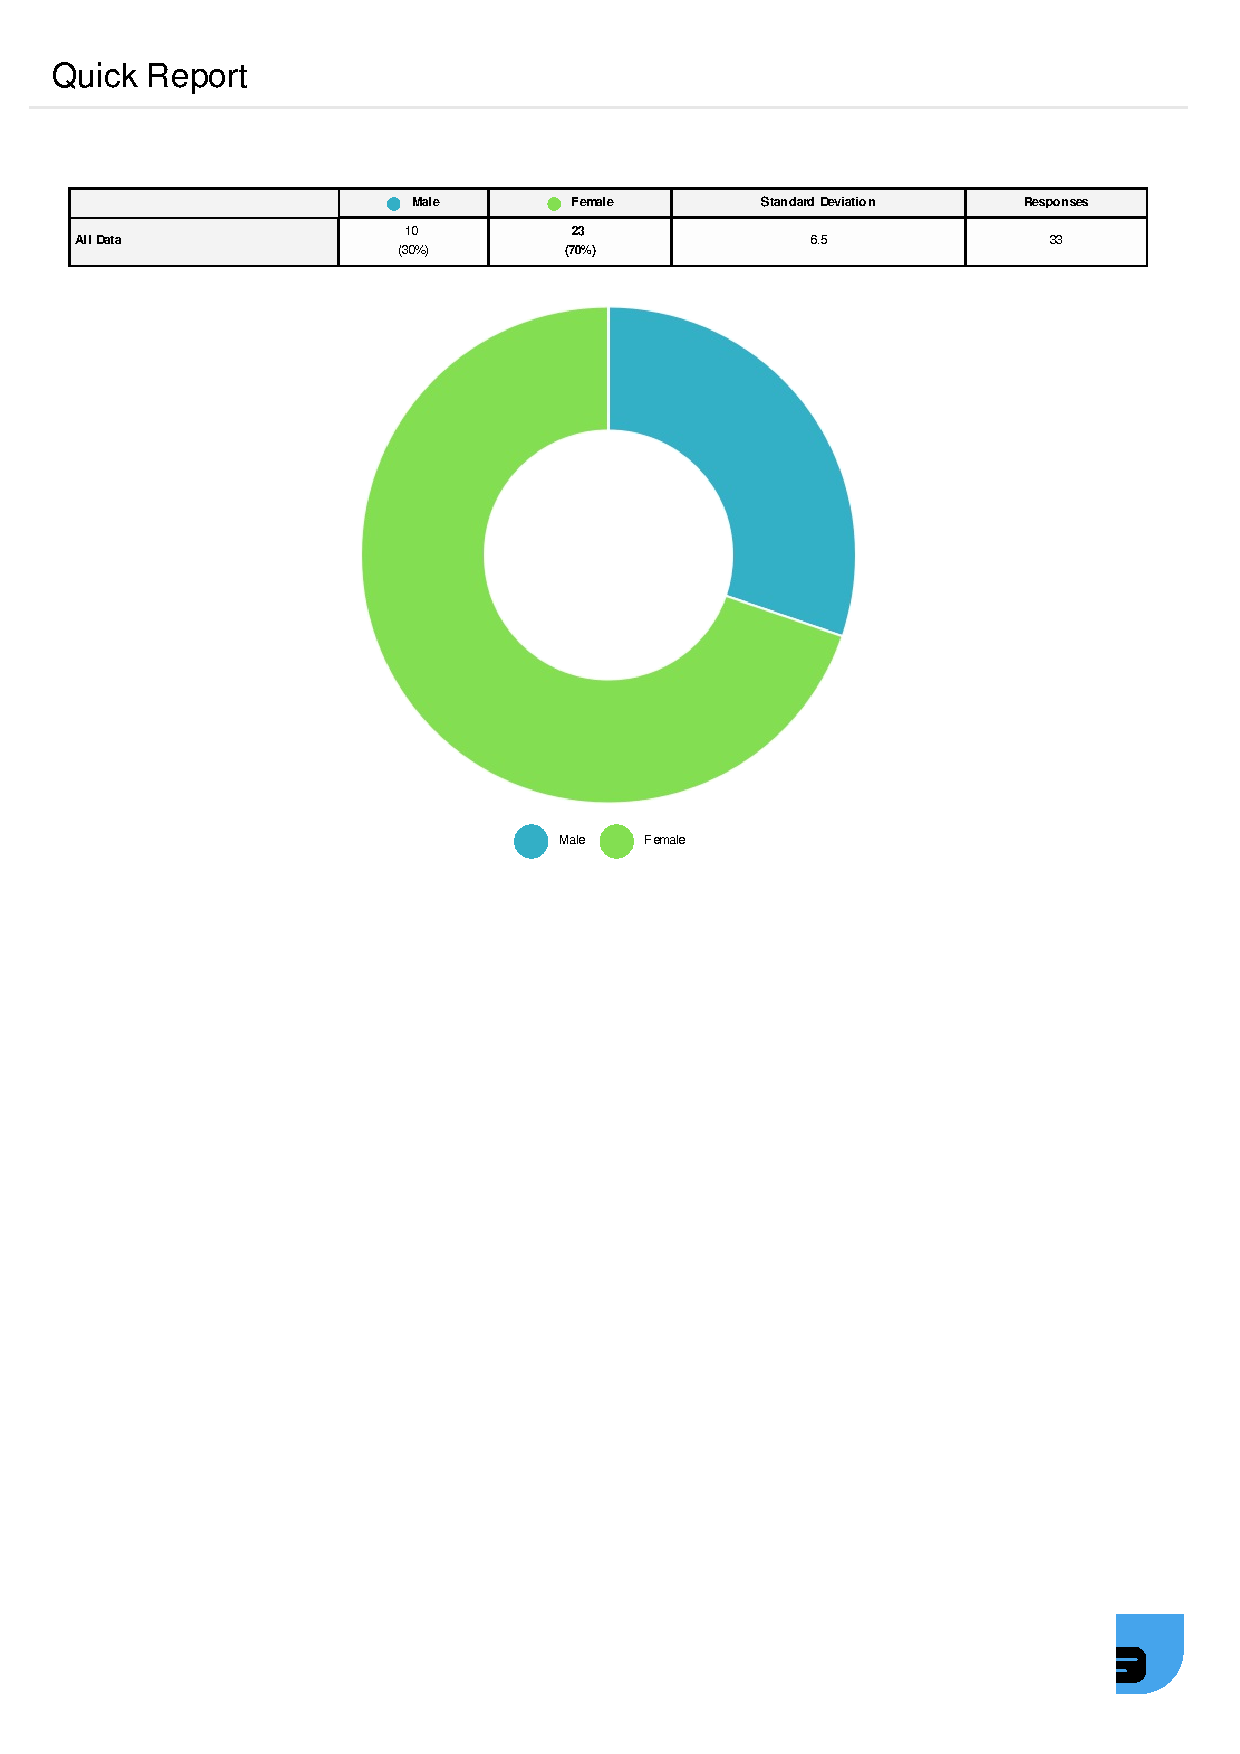
\includepdf[pages=-]{usergapsurvey.pdf}
\chapter{Functionality Analysis}

\section{Functionality analysis methodology}
A functionality analysis looks at how well an application meets the requirements of the user. A high level programming like C++ or Python is very functional, but is not usable without considerable time and developmental resources. While a programming language could meet the user's need - eventually - but it is impractical to use, especially if a rapid solution is needed.

Software being used to meet current EPL requirements were measured using six criteria:

\begin{itemize}
\item \textbf{Enterprise} measured whether the application was deployed on a server for shared access or installed on a personal workstation only. Enterprise applications received a 1, while desktop applications received a -1. 
\item \textbf{Metadata} measured the applications ability to accept and store metadata and secondary information such as chain of custody and user access. Systems that could handle or collect metadata received a 1 while systems that coudl not received -1.
\item \textbf{Configured} measured how well the application could be customized to local users needs. A configurable system that was tailored to specific KEPA requirement and country specific parameters received a 1. Non configurable systems for general use received a -1. It could be argued that Excel is configurable, however it would require considerable effort to design a specific application from it, in which case it would not be Excel, but an Excel application.
\item \textbf{Raw Data} evaluated the ability of the system to receive raw data and process it before using it for reports. Allows for the ability to check data for errors and produce TCD. A system that could receive raw data was awarded a 1, a system that could not received -1. Systems that could handle some forms of raw data received a 0.
\item \textbf{Search} described the ability of the application to search for specific records and past datasets. Systems with search or query functions received a 1 while systems without received -1.
\item \textbf{Completeness} measured the built in functionality specific to the requirement. Completeness is for individual systems is described below in Table \ref{completeness}. Systems with full functionality relative to EPL requirements received a 2, while systems that had partial requirements received a 1 or 0. Systems that did not meet any requirements received a -1.
\end{itemize}

The individual scores for each category were summed for a total score. Functionality assessment was awarded based on the the total score as shown in Table \ref{tab:funcrange}.

\begin{table}[H]
\centering
\caption{Functionality range for existing EIS applications}
\label{tab:funcrange}
\begin{tabular}{@{}lc@{}}
\toprule
\textbf{Functionality} & \textbf{Range} \\ \midrule
Functionally complete (Yes) & 7 - 5 \\
Partially complete (Partial) & 4 - -1 \\
Does not meet requirements (No) & -2 - -6 \\ \bottomrule
\end{tabular}
\end{table}

The results of the Functionality analysis is shown in Table \ref{tab:FuncAnalysisEPL}. 


%%%%%%%%%%%%%%% rotate page for big table

\begin{landscape}

\begin{table}[H]
\centering
\caption{Functional analysis of implied EIS requirements and existing EIS applications}
\label{tab:FuncAnalysisEPL}
\resizebox{\columnwidth}{!}{%
\begin{tabular}{@{}lccccccccc@{}}
\toprule
\textbf{EIS Requirement} & \textbf{Existing System} & \textbf{Enterprise} & \textbf{Metadata} & \textbf{Configured} & \textbf{Raw Data} & \textbf{Search} & \textbf{Completeness} & \textbf{Score} & \textbf{Functionality} \\ \midrule
Air concentration DB & Envista ARM & 1 & 1 & 1 & 1 & 1 & 2 & 7 & Yes \\
Marine sample DB & EQuIS & 1 & 1 & 1 & 1 & 1 & 2 & 7 & Yes \\
Water sample Mgmt DB & EQuIS & 1 & 1 & 1 & 1 & 1 & 2 & 7 & Yes \\
Air Mgmt DB & AQMIS & 1 & 1 & 1 & 0 & 1 & 2 & 6 & Yes \\
Geospatial DB & ArcGIS & 1 & 1 & 1 & 0 & 1 & 2 & 6 & Yes \\
Land Use/Agriculture registry & ArcGIS & 1 & 1 & 1 & 0 & 1 & 2 & 6 & Yes \\
Land Use/Camp ground registry & ArcGIS & 1 & 1 & 1 & 0 & 1 & 2 & 6 & Yes \\
Land Use/Coastal registry & ArcGIS & 1 & 1 & 1 & 0 & 1 & 2 & 6 & Yes \\
Land Use/Natural Resources & ArcGIS & 1 & 1 & 1 & 0 & 1 & 2 & 6 & Yes \\
Land Use/Plant registry & ArcGIS & 1 & 1 & 1 & 0 & 1 & 2 & 6 & Yes \\
Land Use/Quarry registry & ArcGIS & 1 & 1 & 1 & 0 & 1 & 2 & 6 & Yes \\
ODS Mgmt DB & ESS & 1 & 1 & 1 & 0 & 1 & 0 & 4 & Partial \\
Compliance DB & Violations & 1 & 0 & 1 & -1 & 1 & 0 & 2 & Partial \\
Statistical Analysis & Excel & -1 & 0 & -1 & 1 & -1 & 1 & -1 & Partial \\
Building Database & Excel & -1 & 0 & -1 & 1 & -1 & 0 & -2 & No \\
LIMS & Excel & -1 & 0 & -1 & 1 & -1 & 0 & -2 & No \\
Chemical Mgmt DB & Excel & -1 & 0 & -1 & 1 & -1 & -1 & -3 & No \\
Energy Mgmt DB & Excel & -1 & 0 & -1 & 1 & -1 & -1 & -3 & No \\
Incident Mgmt DB & Excel & -1 & 0 & -1 & 1 & -1 & -1 & -3 & No \\
Noise Mgmt DB & Excel & -1 & 0 & -1 & 1 & -1 & -1 & -3 & No \\
Nuclear Waste Mgmt DB & Excel & -1 & 0 & -1 & 1 & -1 & -1 & -3 & No \\
Organism Mgmt DB & Excel & -1 & 0 & -1 & 1 & -1 & -1 & -3 & No \\
Waste Mgmt DB & Excel & -1 & 0 & -1 & 1 & -1 & -1 & -3 & No \\ \bottomrule
\end{tabular}
}%end resize
\end{table}

\end{landscape}

\section{Completeness score}
The Completeness score was determined by assigning functional criteria to each requirement and scoring the requirement with a 1 (meets the requirement) or 0 (does not meet the requirement). The criteria scores are added up and compared to the maximum score (total number of criteria).  The percentage of the score to the maximum forms the basis of award as shown below where $x$ is the percentage of the score divided by the maximum value.

\centering
\begin{tabular}{l}
$x = 100\% \rightarrow 2$ \\
$100\% <x \ge50\% \rightarrow 1$ \\
$0<x <50\%\rightarrow 0 $\\
$x=0\rightarrow -1$
\end{tabular}


The Completeness scores are shown in Table \ref{tab:completeness}.

\begin{table}[H]
\centering
\caption{Calculation of Completeness score for Functionality Analysis}
\label{tab:completeness}
\resizebox{\columnwidth}{!}{%
\begin{tabular}{@{}cclccc@{}}
\toprule
\textbf{Requirement} & \textbf{Existing SW} & \textbf{Functionality} & \textbf{Score} & \textbf{Max} & \textbf{Rating} \\ \midrule
Air Mgmt DB & AQMIS & Emission unit level emissions inventory & 1 &  &  \\
Air Mgmt DB & AQMIS & Add/update emission factors for specific chemical and process & 1 &  &  \\
Air Mgmt DB & AQMIS & Calculate wide area dispersion models & 1 &  &  \\
Air Mgmt DB & AQMIS & Quantified risk assessments & 1 &  &  \\
Air Mgmt DB & AQMIS & Map sources and receptors & 1 &  &  \\
Air Mgmt DB & AQMIS & Report by specific criteria & 1 &  &  \\
Air Mgmt DB & AQMIS & Display air station data & 1 &  &  \\
 &  & Air Mgmt DB completeness score & 7 & 7 & 2 \\
 &  &  &  &  &  \\
Geospatial DB & ArcGIS & Add/Update attribute tables & 1 &  &  \\
Geospatial DB & ArcGIS & Associate different data sets with geospatial locations & 1 &  &  \\
Geospatial DB & ArcGIS & Receive time series data sets & 1 &  &  \\
 &  & Geospatial DB completeness score & 3 & 3 & \textbf{2} \\
 &  &  &  &  &  \\
Land Use/Agriculture registry & ArcGIS & Associate land use categories with geospatial locations & 1 &  &  \\
 &  & Land Use/Agriculture registry completeness score & 1 & 1 & \textbf{2} \\
 &  &  &  &  &  \\
Land Use/Camp ground registry & ArcGIS & Associate designate  with geospatial locations & 1 &  &  \\
 &  & Land Use/Camp ground registry completeness score & 1 & 1 & \textbf{2} \\
 &  &  &  &  &  \\
Land Use/Coastal registry & ArcGIS & Associate coastlines with geospatial locations & 1 &  &  \\
Land Use/Coastal registry & ArcGIS & Link structures with contact information and responsible party & 1 &  &  \\
Land Use/Coastal registry & ArcGIS & Allow for coast profiles and change analysis & 1 &  &  \\
 &  & Land Use/Coastal registry completeness score & 3 & 3 & \textbf{2} \\
 &  &  &  &  &  \\
Land Use/Natural Resources & ArcGIS & Associate land use categories with geospatial locations & 1 &  &  \\
 &  & Land Use/Natural Resources completeness score & 1 & 1 & \textbf{2} \\
 &  &  &  &  &  \\
Land Use/Plant registry & ArcGIS & Associate land use categories with geospatial locations & 1 &  &  \\
 &  & Land Use/Plant registry completeness score & 1 & 1 & \textbf{2} \\
 &  &  &  &  &  \\
Land Use/Quarry registry & ArcGIS & Associate quarry locations and ownership with geospatial locations & 1 &  &  \\
 &  & Land Use/Quarry registry completeness score & 1 & 1 & \textbf{2} \\
 &  &  &  &  &  \\
Air concentration DB & Envista ARM & Log time series of multiple data streams from different locations & 1 &  &  \\
Air concentration DB & Envista ARM & Provide search and query features to locate specific data sets & 1 &  &  \\
 &  & Air concentration DB completeness score & 2 & 2 & \textbf{2} \\
 &  &  &  &  &  \\
Marine sample DB & Excel & Capture sample collection metadata and analytical results & 1 &  &  \\
Marine sample DB & Excel & Associate collected samples with physical location & 1 &  &  \\
Marine sample DB & Excel & Provide search and query features to locate specific data sets & 1 &  &  \\
 &  & Marine sample DB completeness score & 3 & 3 & \textbf{2} \\
 &  &  &  &  &  \\
Water sample Mgmt DB & Excel & Capture sample collection metadata and analytical results & 1 &  &  \\
Water sample Mgmt DB & Excel & Associate collected samples with physical location & 1 &  &  \\
Water sample Mgmt DB & Excel & Provide search and query features to locate specific data sets & 1 &  &  \\
 &  & Water sample Mgmt DB completeness score & 3 & 3 & \textbf{2} \\
 &  &  &  &  &  \\
ODS Mgmt DB & ESS & Track export/import of ODS materials & 1 &  &  \\
ODS Mgmt DB & ESS & List and search companies exporting and importing ODS material & 1 &  &  \\
ODS Mgmt DB & ESS & Track training of certified technicians & 0 &  &  \\
ODS Mgmt DB & ESS & Track consumption of ODS & 0 &  &  \\
 &  & ODS Mgmt DB completeness score & 2 & 4 & \textbf{0} \\
 &  &  &  &  &  \\
Building Database & Excel & Track facility location and owner & 1 &  &  \\
Building Database & Excel & Track industrial code and process & 0 &  &  \\
 &  & Building Database completeness score & 1 & 2 & \textbf{0} \\
 &  &  &  &  &  \\
Chemical Mgmt DB & Excel & Track export/import of hazardous materials & 1 &  &  \\
Chemical Mgmt DB & Excel & Track bulk storage areas & 0 &  &  \\
Chemical Mgmt DB & Excel & Track approved chemicals and hazardous materials & 0 &  &  \\
 &  & Chemical Mgmt DB completeness score & 1 & 3 & \textbf{0} \\
 &  &  &  &  &  \\
Incident Mgmt DB & Excel & Allow different type of incidents & 0 &  &  \\
Incident Mgmt DB & Excel & Capture location, materials involved, associated parties & 0 &  &  \\
Incident Mgmt DB & Excel & Allow for follow-up action tracking & 0 &  &  \\
Incident Mgmt DB & Excel & Attach pictures and documents & 0 &  &  \\
 &  & Incident Mgmt DB completeness score & 0 & 4 & \textbf{-1} \\
 &  &  &  &  &  \\
Noise Mgmt DB & N/A & Capture noise profiles for areas & 0 &  &  \\
Noise Mgmt DB & N/A & Associate noise sources with locations & 0 &  &  \\
Noise Mgmt DB & N/A & Track complaints by location, processes, and timestamp & 0 &  &  \\
 &  & Noise Mgmt DB completeness score & 0 & 3 & \textbf{-1} \\
 &  &  &  &  &  \\
Nuclear Waste Mgmt DB & Excel & Register authorized user, suppliers, transporters and disposal facilities & 1 &  &  \\
Nuclear Waste Mgmt DB & Excel & Track movement and disposal of wastes by type & 0 &  &  \\
 &  & Nuclear Waste Mgmt DB completeness score & 1 & 2 & \textbf{1} \\
 &  &  &  &  &  \\
Waste Mgmt DB & Excel & Register authorized user, suppliers, transporters and disposal facilities & 1 &  &  \\
Waste Mgmt DB & Excel & Track movement and disposal of wastes by type & 0 &  &  \\
 &  & Waste Mgmt DB completeness score & 1 & 2 & \textbf{1} \\
 &  &  &  &  &  \\
Organism Mgmt DB & Excel & Capture sample collection metadata and analytical results & 1 &  &  \\
Organism Mgmt DB & Excel & Associate collected samples with physical location & 0 &  &  \\
Organism Mgmt DB & Excel & Provide search and query features to locate specific data sets & 0 &  &  \\
 &  & Organism Mgmt DB completeness score & 1 & 3 & \textbf{0} \\
 &  &  &  &  &  \\
LIMS & Excel & Track instrument calibration and usage & 1 &  &  \\
LIMS & Excel & Track analyte expiration dates & 0 &  &  \\
LIMS & Excel & Track chain of custody of samples & 0 &  &  \\
LIMS & Excel & Capture results and associated metadata & 1 &  &  \\
LIMS & Excel & Prepare reports in EDD formats & 0 &  &  \\
 &  & LIMS completeness score & 2 & 5 & \textbf{0} \\
 &  &  &  &  &  \\
Statistical Analysis & Excel & Provide easy import of different data file formats & 1 &  &  \\
Statistical Analysis & Excel & Have standard descriptive statistical and transformation functions and graph capabilities & 1 &  &  \\
Statistical Analysis & Excel & Have statistical test functions & 0 &  &  \\
 &  & Statistical Analysis completeness score & 2 & 3 & \textbf{1} \\
 &  &  &  &  &  \\
Compliance DB & Violations & Capture violation fines & 1 &  &  \\
Compliance DB & Violations & Track permit and facility operating conditions & 0 &  &  \\
Compliance DB & Violations & Track past violations by facility & 0 &  &  \\
Compliance DB & Violations & Track findings and assign responsibilities & 0 &  &  \\
Compliance DB & Violations & Assign article or regulation to finding & 0 &  &  \\
 &  & Compliance DB completeness score & 1 & 5 & \textbf{0} \\ \bottomrule
\end{tabular}
}%end resize
\end{table}
\chapter{KEDD Spill and Waste fields}


\begin{table}[H]
\centering
\resizebox{\columnwidth}{!}{%
\begin{tabular}{@{}llll@{}}
\toprule
Spill reporting sheet & Waste generator sheet & Waste Transport Sheet & Waste Receiver sheet \\ \midrule
\#MANID & \#MANID & \#MANID & \#MANID \\
G\_SPILL\_LAT & G\_POC\_NAME & T\_TRANS\_ID & R\_RECV\_ID \\
G\_SPILL\_LONG & G\_POC\_PHONE & T\_DRIVER & R\_POC\_NAME \\
G\_SPILL\_DATE & G\_POC\_EMAIL & T\_DRIVERID & R\_POC\_PHONE \\
G\_SPILL\_AREA & G\_WM\_TYPE & T\_DRIVER\_PHONE & R\_POC\_EMAIL \\
G\_SPILL\_AREA\_UNITS & G\_WM\_OTHER & T\_VEHLIC & R\_RECVTEST \\
G\_SPILL\_MAT & G\_STREAM & T\_VEHCAP & R\_RECVRESULTS \\
G\_SPILL\_QTY & G\_SOURCE & T\_VEHCAP\_UNITS & R\_RECVRESULTS\_UNITS \\
G\_SPILL\_QTY\_UNITS & G\_EXP & T\_VEHEMPTWGHT & R\_REJECTED \\
G\_SPILL\_POC & G\_FLAM & T\_TOTWGHT & R\_REJECTREASON \\
G\_SPILL\_PHONE & G\_REACT & T\_TOTWGHT\_UNITS & R\_DATERECVD \\
 & G\_CORR & T\_PICKUP\_DATE & R\_TREAT\_TYPE \\
 & G\_POIS & R\_REJECTED & R\_TREAT\_OTHER \\
 & G\_RAD & R\_REJECTREASON & R\_TREAT\_DATE \\
 & G\_OTHER & T\_DATERETURN & R\_AMT\_TREATED \\
 & G\_CONT\_TYPE &  & R\_AMT\_TREATED\_UNITS \\
 & G\_NUM\_CONT &  & R\_DISPOSAL\_TYPE \\
 & G\_CONT\_LAT &  & R\_DISPOSAL\_OTHER \\
 & G\_CONT\_LONG &  & R\_TOTDISPOSED \\
 & G\_WASTE\_WGHT &  & R\_TOTDISPOSED\_UNITS \\
 & G\_WASTE\_WGHT\_UNITS &  & R\_TOTRECYCLED \\
 & G\_GEN\_DATE &  & R\_TOTRECYCLED\_UNITS \\
 & G\_SCHED\_DATE &  & R\_DISPOSAL\_DATE \\
 & G\_DISPATCH\_DATE\_TIME &  & R\_RECYCLE\_ID \\ \bottomrule
\end{tabular}
} %end resize
\end{table}
\end{appendices}


\end{document}  